\documentclass[oneside,a4paper,12pt]{book}

\usepackage[lmargin=2.8cm, rmargin=2.8cm, tmargin=3.3cm, bmargin=3.3cm]{geometry}
\usepackage{caption}
\usepackage{graphicx}
\usepackage[utf8]{inputenc}
\usepackage[spanish]{babel}
\usepackage{float}
\usepackage{listings}
\usepackage{color}

\usepackage{minted}
\usemintedstyle{borland}

\graphicspath{ {img/} }

\renewcommand{\baselinestretch}{1}

\definecolor{backcolour}{rgb}{0.95,0.95,0.92}
\definecolor{gray}{rgb}{.4,.4,.4}

\lstdefinelanguage{JSON}{
    string=[s]{"}{"},
    stringstyle=\color{blue},
    comment=[l]{:},
    commentstyle=\color{red}  
}

\lstdefinelanguage{JavaScript}{
  backgroundcolor = \color{backcolour},
  keywords={typeof, function, var, if},
  keywordstyle=\color{red}\bfseries,
  comment=[l]{//},
  commentstyle=\color{gray}\ttfamily
  stringstyle=\color{red}\ttfamily,
  morestring=[b]',
  morestring=[b]"
}

\lstset{
    language = JSON,
    backgroundcolor = \color{backcolour},
    basicstyle=\footnotesize\ttfamily,
    showstringspaces=false,
    showspaces=false,
    frame=single,
    tabsize=2,
    breaklines=true,
    showtabs=false,
    captionpos=b
}

\begin{document}

\chapter{Introducción}
\section{La evolución de las aplicaciones web }
\subsection{Las primeras webs (web 1.0)}
Actualmente la web se ha convertido en algo cotidiano entre los mas de 600 millones de usuarios que componen internet, suponiendo un impacto en la economía mundial incalculable. Todo empezó en 1990 cuando Tim Bermers-Lee creó lo que hoy concebimos como web 1.0, una versión inicial de la web que nada tiene que ver con lo que conocemos hoy en día. 

Nace como un sistema de hipertexto para compartir información en internet, con la finalidad de publicar documentos. Cuando las empresas empiezan a darse cuenta del potencial de la web, empiezan a incorporar información corporativa con la finalidad de ser más próximos a los clientes y como un canal mas para promocionarse. Pero pronto se dan cuenta de las limitaciones que la web 1.0 contiene:

\begin{itemize}

    \item El contenido publicado no se actualizaba constantemente por lo que podían pasar largos periodos de tiempo sin que esa información se modificase.

    \item Las páginas eran estáticas y no permitían interacción de ningún tipo

    \item La principal desventaja es que eran difícil de manejar y solo podían publicar contenido los más entendidos en el tema o web masters.
 
\end{itemize}


\begin{figure}[H]
    \centering
    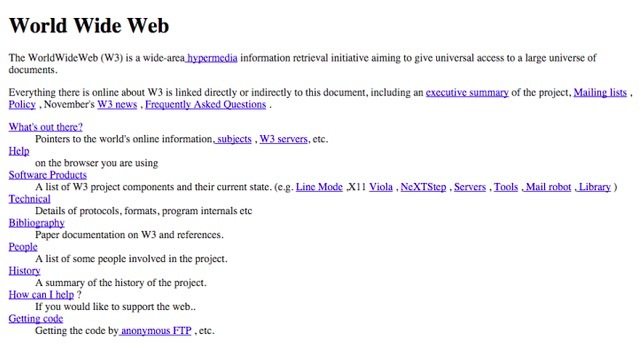
\includegraphics[width=80mm]{memoria/LaTeX/img/introduccion/web1.jpg}
    \caption[Ejemplo web 1º generación]{Ejemplo web 1º generación}
\end{figure}

\subsection{Las primeras app web (web 2.0)}

Debido a las limitaciones que ofrece la web 1.0, nace una nueva forma de concebir la web donde se valora las reacciones de los usuarios. Surgen aplicaciones y páginas que utilizan la inteligencia colectiva, consecuencia de ello las páginas pueden ser personalizadas convirtiéndose en una herramienta dinámica que permite el intercambio de información. Es por eso que la información se transforma en comunicación gracias a la interacción y a la incorporación de textos, vídeos, chats… Con esta nueva forma de concebir la web nacen los blogs, las redes sociales, los wikis … Este cambio ha supuesto una gran revolución, puesto que permite devolver la información de los usuarios y poder procesarla con el objetivo de controlar mejor la demanda. 


\begin{figure}[H]
    \centering
    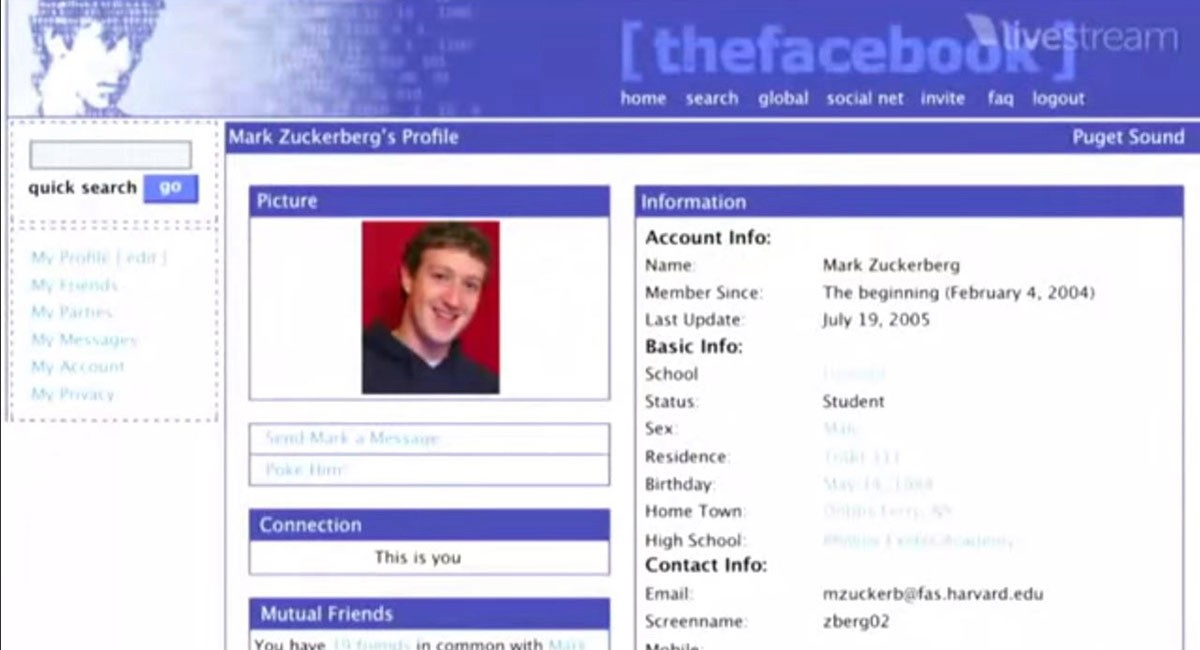
\includegraphics[width=80mm]{memoria/LaTeX/img/introduccion/web2.jpeg}
    \caption{Ejemplo web 2º generación}
\end{figure}
\subsection{Las app web de hoy en día}

La conocida web 3.0 dará paso a otro tipo de web donde pondrá su objetivo en la inteligencia artificial, un método para que los usuarios puedan no solo encontrar la información sino comprenderla. Este control esta en manos de motores informáticos y procesadores de información, que tratan de analizar nuestro perfil y nuestra actividad en red para enviarnos información de nuestro interés. 
Es por esto que la web 3.0 es definida por el concepto "personalización", ya que pretende devolver al usuario una información lo más afinada posible, filtrada a sus gustos y preferencias, evitando información que no sea de su interés.

\begin{figure}[H]
    \centering
    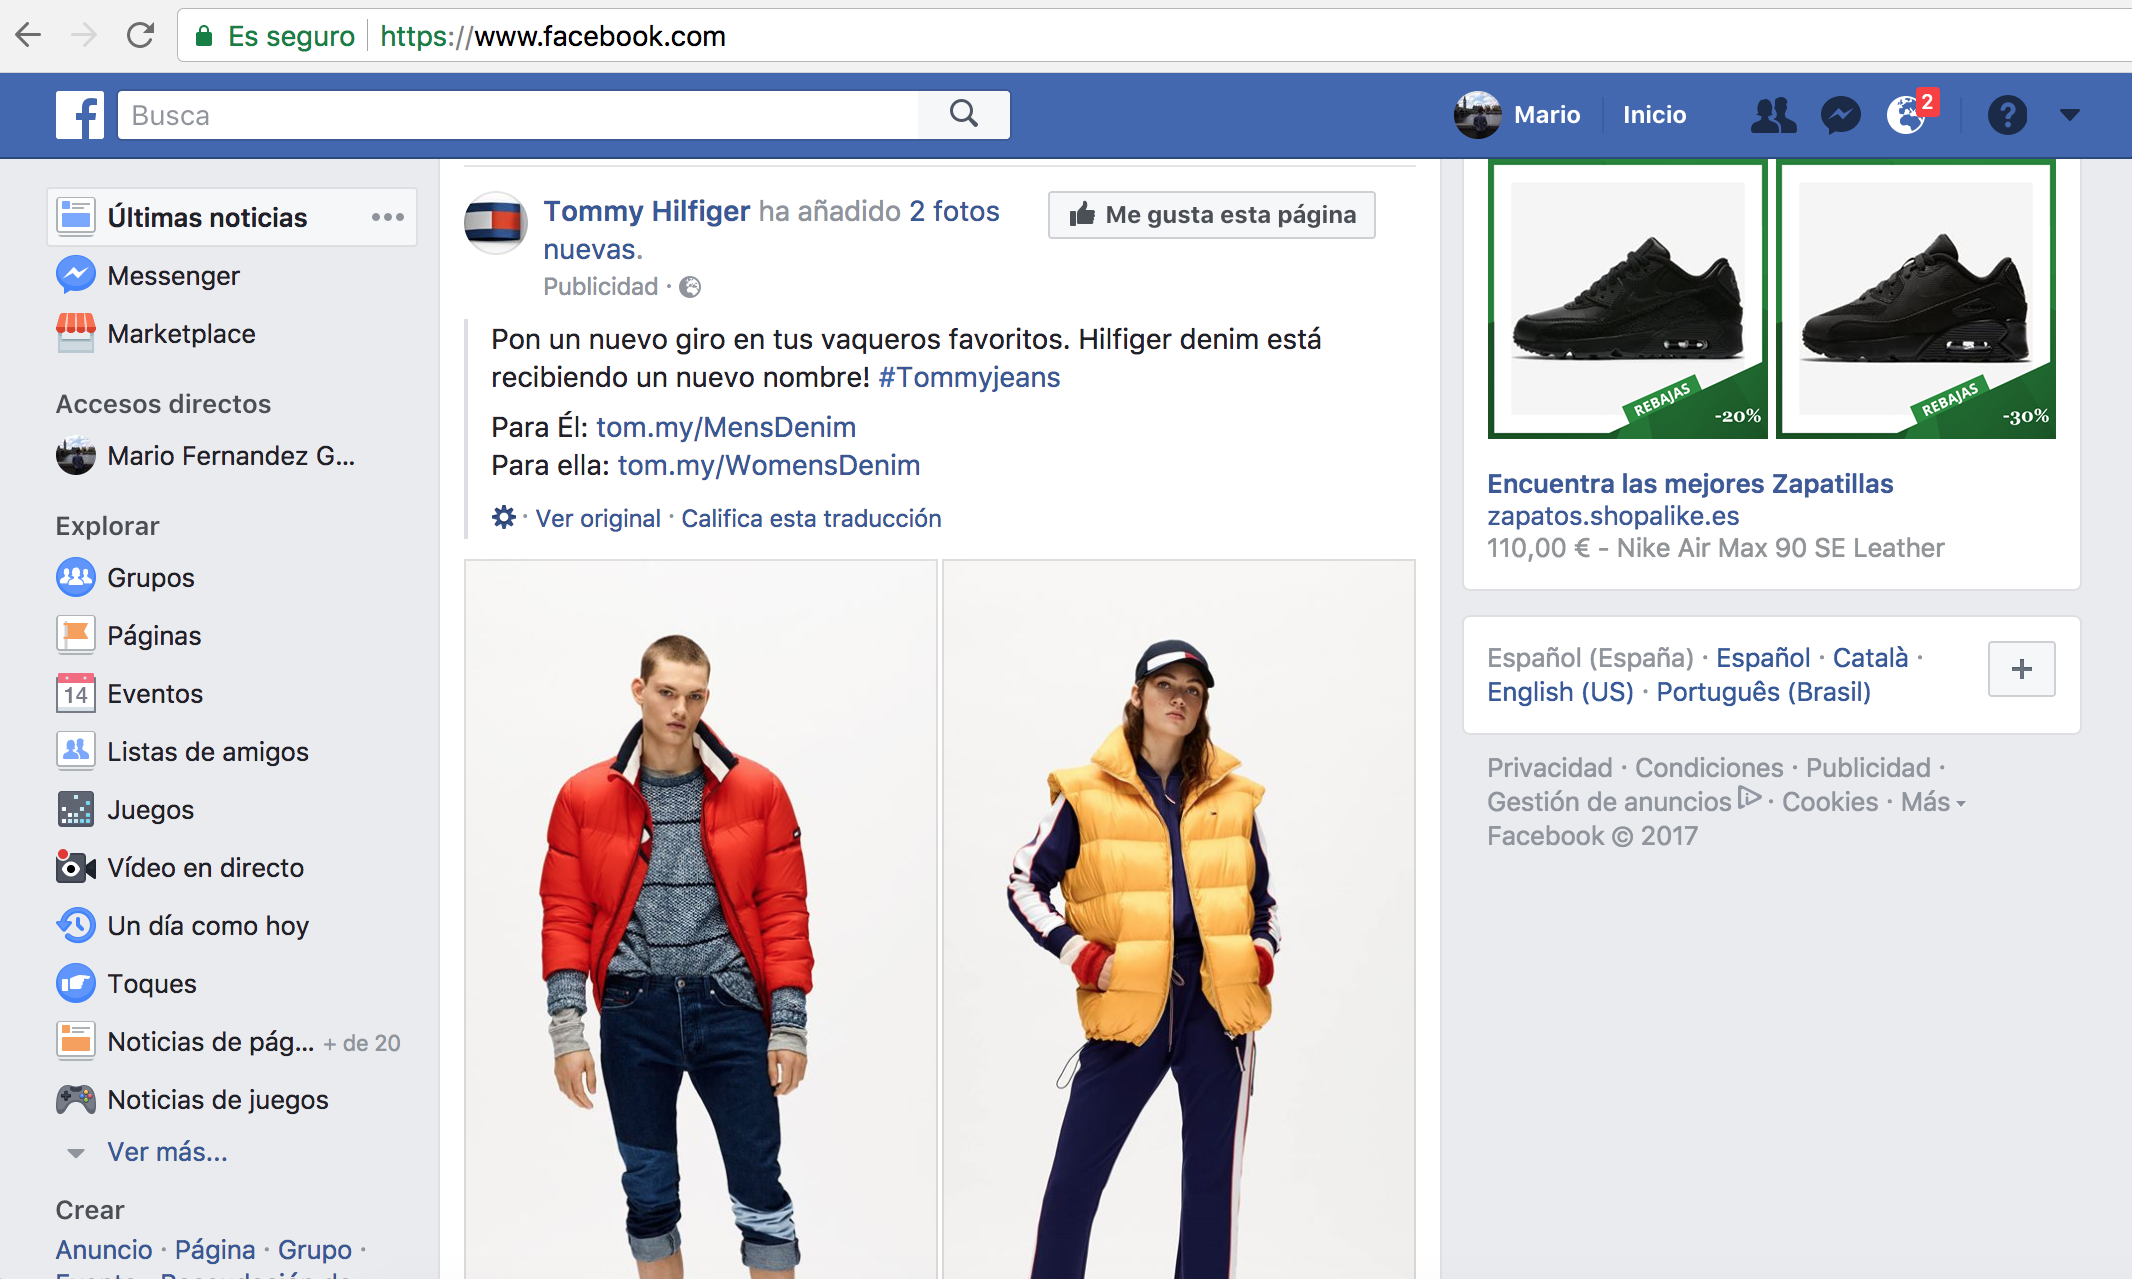
\includegraphics[width=80mm]{memoria/LaTeX/img/introduccion/facebook.png}
    \caption{Ejemplo web 3º generación}
\end{figure}

Con la aparición de la web 3.0, nuevos términos tecnológicos aparecen como:
\begin{itemize}
     \item \textbf{Web SPA: }Una web SPA es una aplicación de una sola página en la que la carga de datos es asíncrona y la página no se recarga en casi ningún momento, pese a cambiar de ruta o url para navegar entre las secciones de la aplicación, es una nueva tendencia en el desarrollo web.
     \item \textbf{Big Data: } Big data o macrodatos es un término que hace referencia a una cantidad de datos tal que supera la capacidad del software convencional para ser capturados, administrados y procesados en un tiempo razonable. El volumen de los datos masivos crece constantemente. En 2012 se estimaba su tamaño de entre una docena de terabytes hasta varios petabytes de datos en un único conjunto de datos.
    \item \textbf{API REST: } El término sirve para describir cualquier interfaz entre sistemas que utilice directamente HTTP para obtener datos o indicar la ejecución de operaciones sobre los datos, en cualquier formato(XML, JSON, etc).
    \begin{figure}[H]
    \centering
    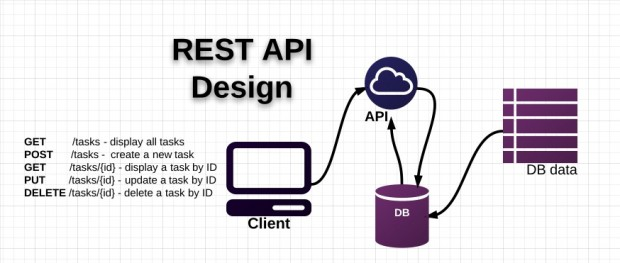
\includegraphics[width=90mm]{memoria/LaTeX/img/introduccion/rest-api.jpg}
    \caption{API-REST}
    \end{figure}
\end{itemize}

\section{Classcity}
\subsection{Objetivo}

Classcity consiste en una aplicación web desarrollada con tecnología de última  generación, cuyo objetivo principal es facilitar el contacto entre alumnos y profesores para dar clases particulares. Classcity utiliza la geolocalización del alumno para proporcionarle los profesores más próximos a él, además de poder filtrar por diferentes parámetros como curso, asignatura y distancia.

\begin{figure}[H]
    \centering
    
\includegraphics[width=40mm]{memoria/LaTeX/img/introduccion/logo.jpg}
\end{figure}

\subsection{Motivación}

Classcity nace motivada por la gran demanda de alumnos que se encuentran con la necesidad de poder encontrar un profesor bien referenciado y que se encuentre próximo al alumno. Es por esto por lo que surge Classcity, una nueva forma de encontrar a tu profesor particular donde el alumno es quien se encarga de buscar al profesor que mas se adapte a sus necesidades.

\subsection{Modelo de negocio}

Aunque no es algo que se haya tenido en cuenta en la implementación del código, Classcity podría tener un modelo de negocio claro.
Cada vez que un alumno concierte una clase con un profesor, se procederá a tramitar el coste de la clase por la aplicación suponiendo que un porcentaje del coste total de la clase vaya destinado al mantenimiento de classcity.
Por otro lado también se podría cobrar a los profesores por una mejor posición en nuestra aplicación, algo así como una cuenta cuenta premium de profesores donde tenga ciertas ventajas sobre las cuentas normales.

\section{Aplicaciones con éxito}


Classcity ha sido desarrollada basándose en modelos de aplicaciones que hoy en día están funcionando, como por ejemplo:

\subsection{Airbnb}

Es una empresa y una plataforma de software dedicada a la oferta de alojamientos a particulares y turísticos. El nombre es un acrónimo de airbed and breakfast (colchón inflable y desayuno). Airbnb tiene una oferta de unas 2.000.000 propiedades en 192 países y 33.000 ciudades. Desde su creación en noviembre de 2008 hasta junio de 2012 se realizaron 10 millones de reservas.

\begin{figure}[H]
    \centering
    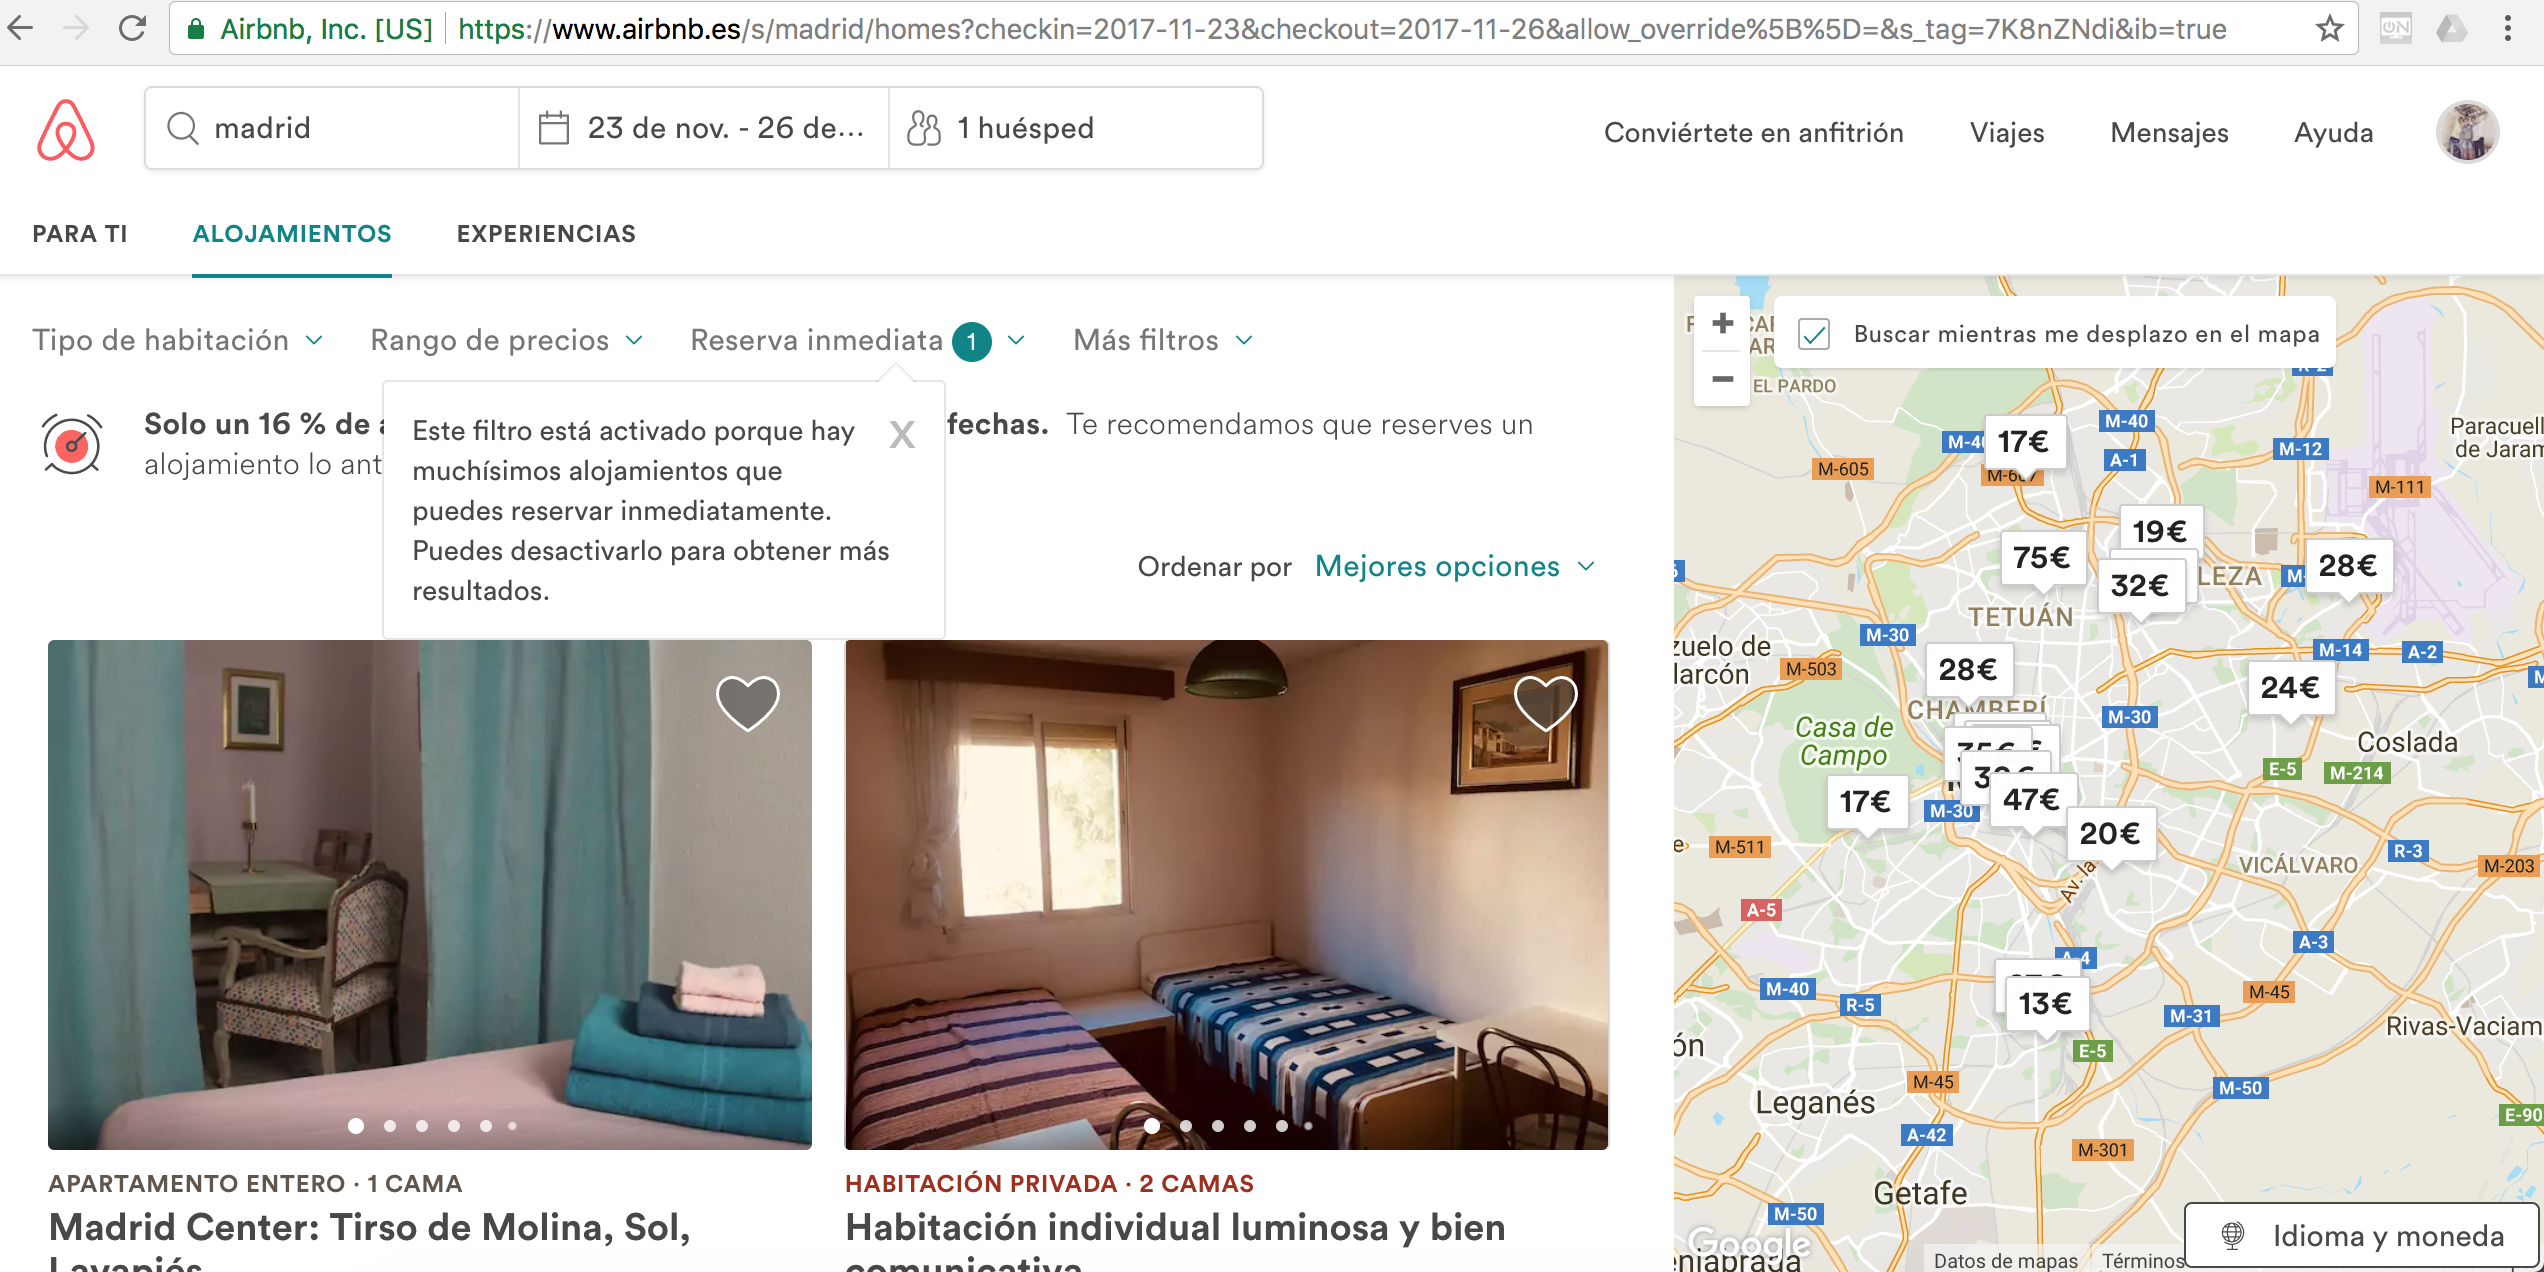
\includegraphics[width=100mm]{memoria/LaTeX/img/introduccion/airbnb.png}
    \caption{Aplicación Airbnb}
\end{figure}

\subsection{Blablacar}

Es un servicio de vehículo compartido que hace posible que las personas que quieren desplazarse al mismo lugar al mismo momento puedan organizarse para viajar juntos. Permite compartir los gastos puntuales del viaje (combustible y peajes) y también evitar la emisión extra de gases de efecto invernadero, al permitir una mayor eficiencia energética en el uso de cada vehículo.

\begin{figure}[H]
    \centering
    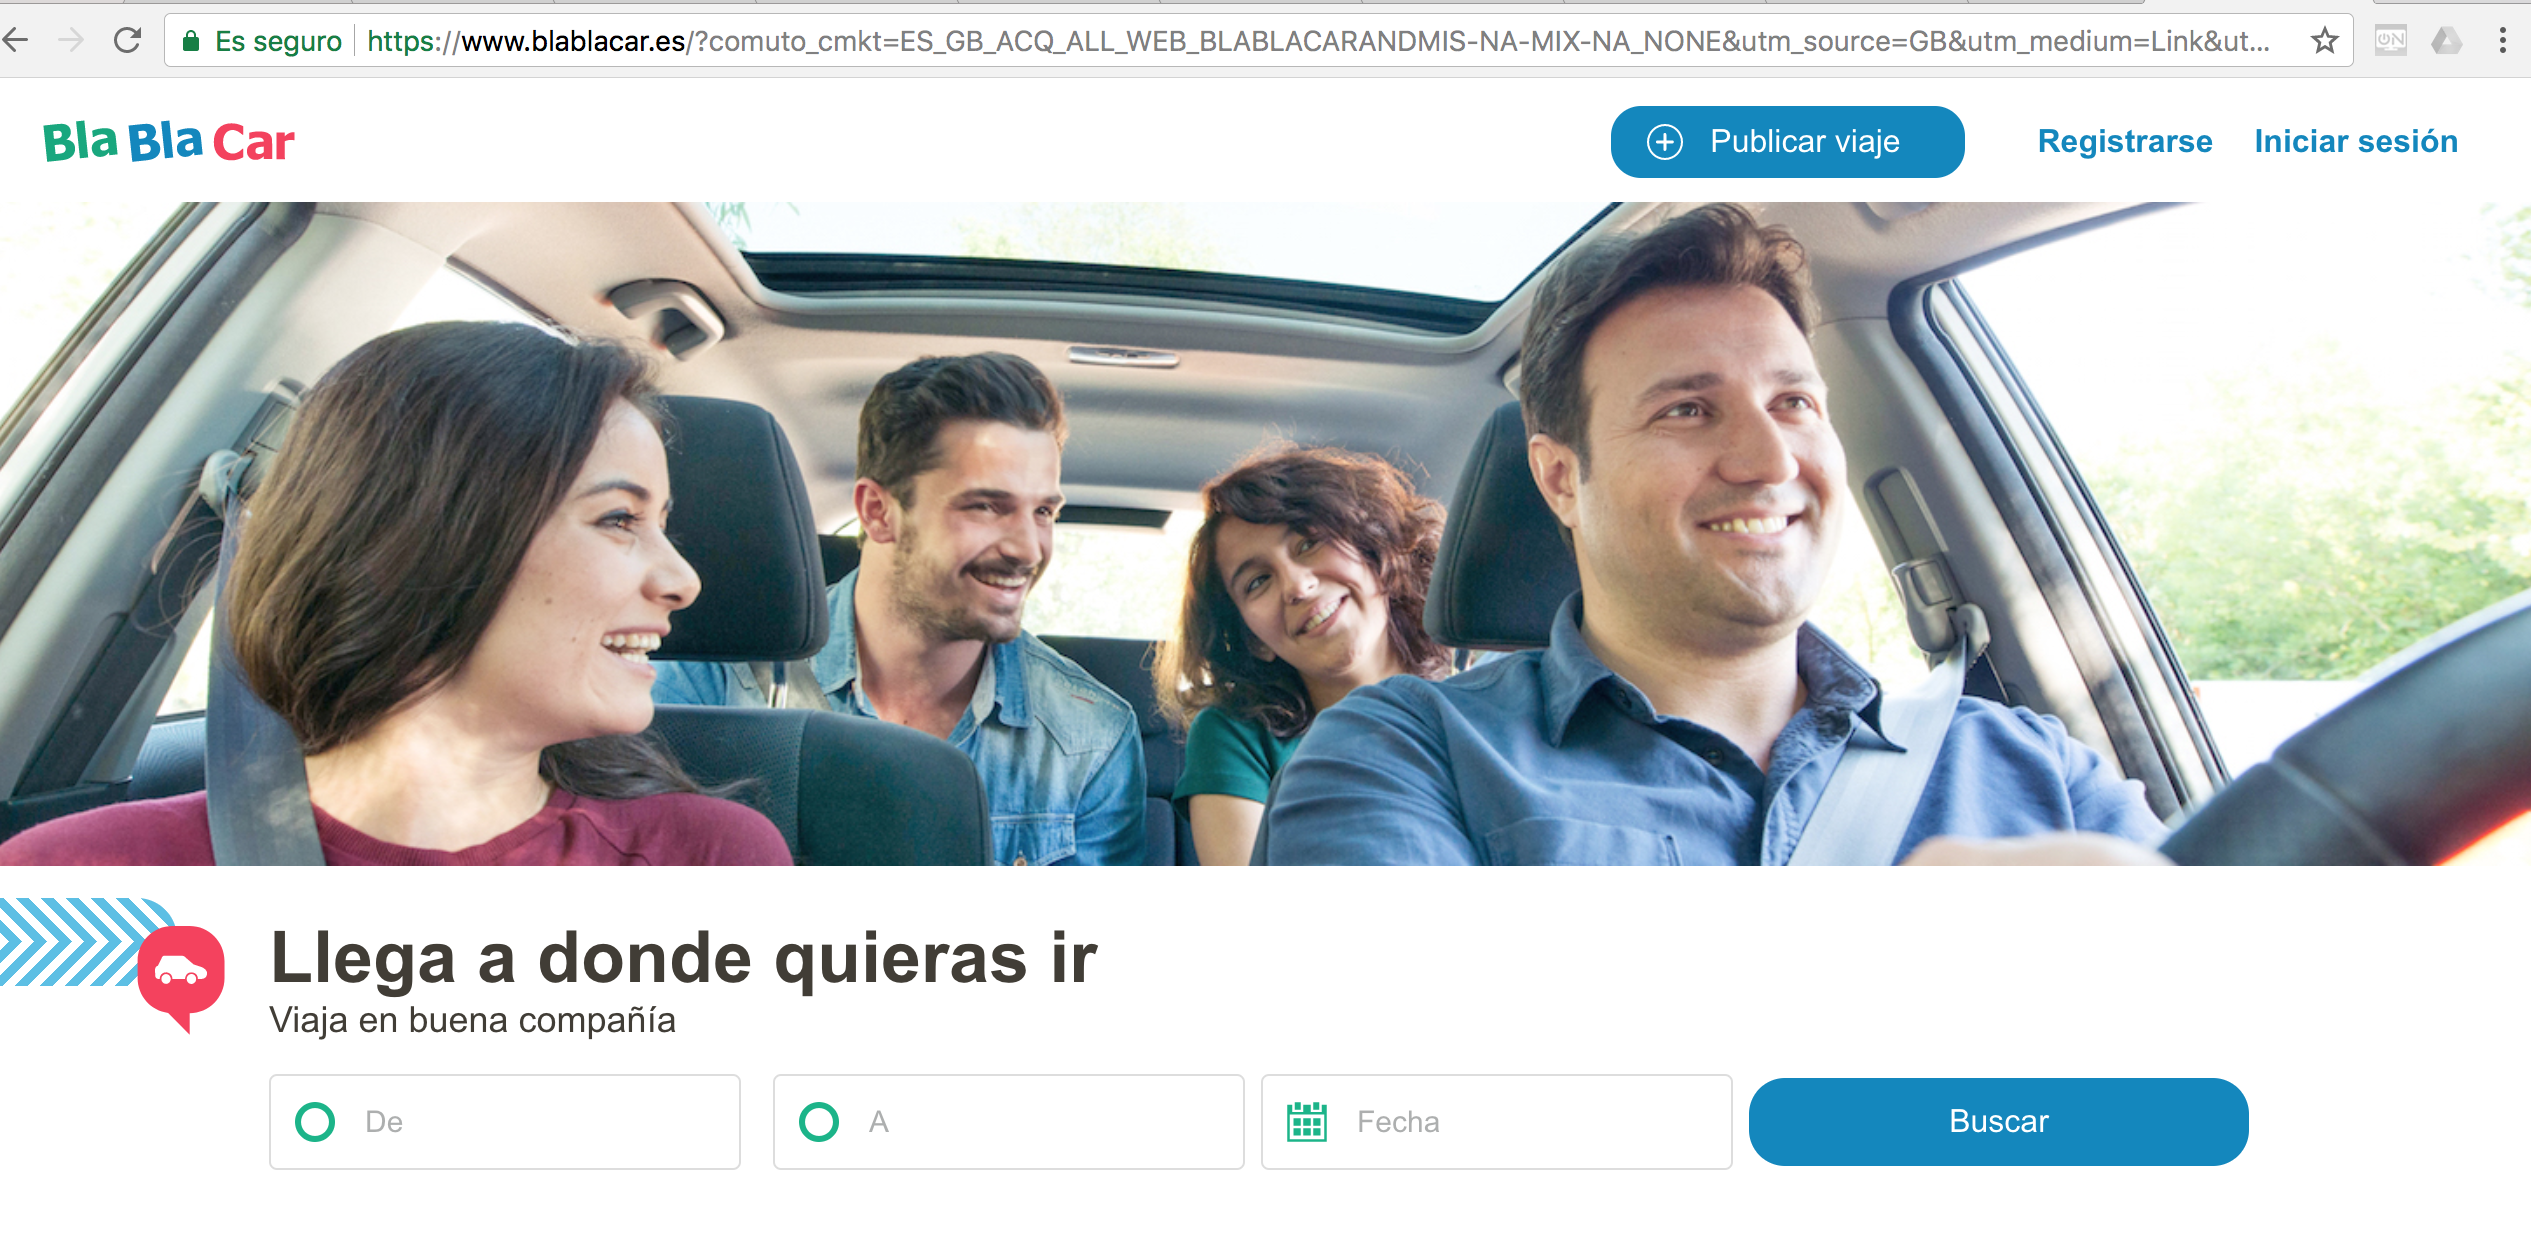
\includegraphics[width=120mm]{memoria/LaTeX/img/introduccion/blablacar.png}
    \caption{Aplicación Blablacar}
\end{figure}

\subsection{Wallapop}

Es una empresa española fundada en 2013, que ofrece un website dedicado a la compra y venta de productos de segunda mano entre usuarios a través de Internet, con un uso centrado en smartphones. Utiliza la geolocalización para que los usuarios puedan comprar y vender en función de su proximidad geográfica

\begin{figure}[H]
    \centering
    
\includegraphics[width=80mm]{memoria/LaTeX/img/introduccion/Wallapop-iPhone.jpg}
    \caption{Aplicación Wallapop}
\end{figure}


\section{Aplicaciones web realizadas en la URJC}

Este TFG centra su desarrollo en técnologias web, es por eso que tanto los proyectos de Edgar Barrero como de Pablo Parejo me han servido para tener una estructura solida de como encaminar mi aplicación web.

\subsection{Suveillance 5.1}

Edgar barrero desarrollo en Ruby sobre Rails Suveillance 5.1, una aplicación web que ofrece un flujo de vídeo desde una cámara web, un flujo de imagen de profundidad procedente de un sector Kinect y su representación en 3D, además de un sensor de humedad y un actuador. 


\begin{figure}[H]
    \centering
    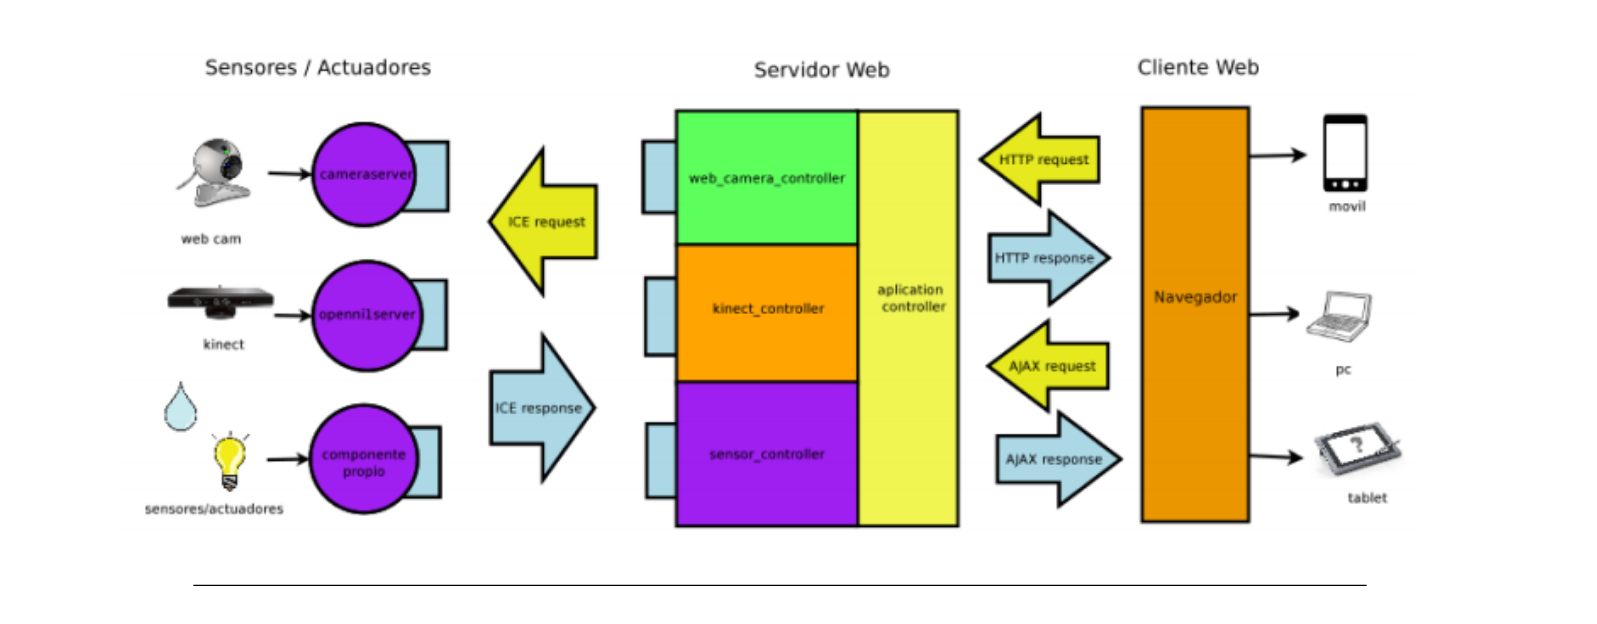
\includegraphics[width=110mm]{memoria/LaTeX/img/introduccion/edgar.png}
    \caption{TFG Edgar Barrero}
\end{figure}

\subsection{Gestión de servicios}
Pablo Parejo desarrollo una aplicación web donde poder gestionar de manera única todos los servicios de almacenamiento en línea que pueda tener un usuario. Aprovechando la oportunidad para adentrarse en tecnologías de última generación como: Angular, CSS3, HTML5, Django...
\begin{figure}[H]
    \centering
    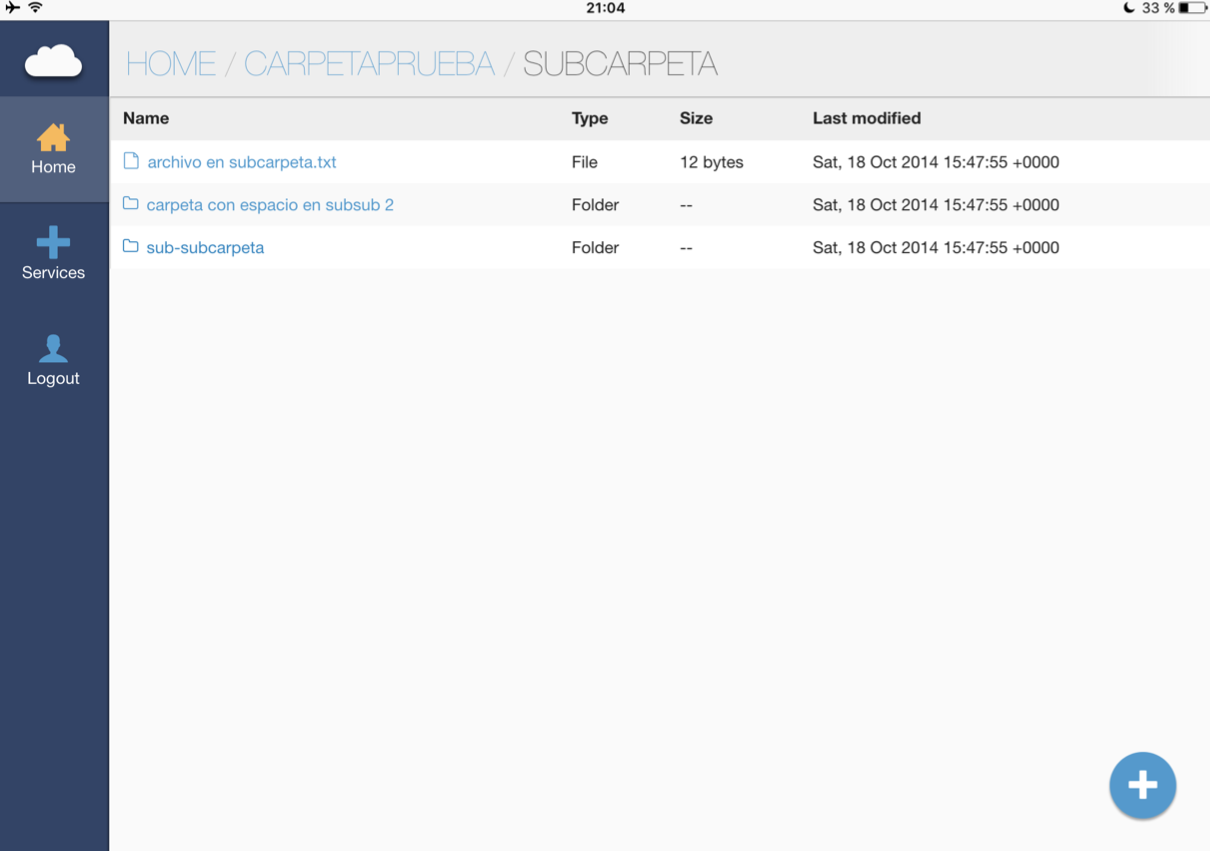
\includegraphics[width=90mm]{memoria/LaTeX/img/introduccion/parejo.png}
    \caption{TFG Pablo Parejo}
\end{figure}















































































































\chapter{Objetivos}
Una vez que hemos enfocado el contexto en el que se va a desarrollar este trabajo, pasamos a definir el objetivo general y los sub-objetivos que se pretender cubrir en este TFG.

El objetivo principal es desarrollar, una aplicación web desarrollada con tecnología de última  generación, cuya funcionalidad es facilitar el contacto entre alumnos y profesores para dar clases particulares. Utilizará la geolocalización del alumno para proporcionarle los profesores más próximos a él, además de poder filtrar por diferentes parámetros como curso, asignatura y distancia.

Para la realización de esta aplicación hemos dividido el objetivo general en cuatro sub-objetivos más sencillos con la finalidad de que quitemos complejidad al proyecto.
\begin{enumerate}

    \item Diseño y desarrollo de la parte del cliente es quizás la más tediosa por su dificultad a la hora de desarrollar una interfaz lo suficientemente ligera y adaptable para diferentes tipos de dispositivo. Es por esto que la elección del entorno en el cliente nos puede cambiar por completo la estructura de nuestra aplicación web, además de reducir mucho los tiempos de desarrollo.

    \item Diseño y desarrollo de la parte servidor de la aplicación web, con de la elección de los diferentes entornos que se adaptan mejor a nuestras necesidades. La elección de este entorno viene condicionado en gran medida por el entorno seleccionado para el cliente. Se programará la lógica de la aplicación en el servidor, incluyendo el establecimiento de chat en vivo.

    \item Habrá que diseñar el modelo de datos adecuado para esta aplicación donde los roles de estudiante y alumno aparecen claros. La base de datos por lo general pueden ser de dos tipos SQL y NoSQL, es por esto que debemos elegir cuál de los dos tipos de bases de datos satisface mas con nuestras necesidades.

    \item Una vez que tengamos nuestra aplicación funcionando correctamente en local, habrá que desplegarla en alguno de las plataformas de computación en la nube que ofrecen lo proveedores más importantes como AWS, Azure o GoogleCloud.


\end{enumerate}
\section{Metodología}
En la realización del proyecto se ha seguido una metodología que permite planificar las tareas necesarias para llegar a nuestro objetivo. El modelo seleccionado para la realización del TFG ha sido de tipo cascada, un proceso de desarrollo secuencial, en el que el desarrollo de software se concibe como un conjunto de etapas que se ejecutan una tras otra. Se le denomina así por las posiciones que ocupan las diferentes fases que componen el proyectom colocadas una encima de otra, y siguiendo un flujo de ejecución de arriba hacia abajo, como una cascada.


\begin{figure}[!h]
    \centering
    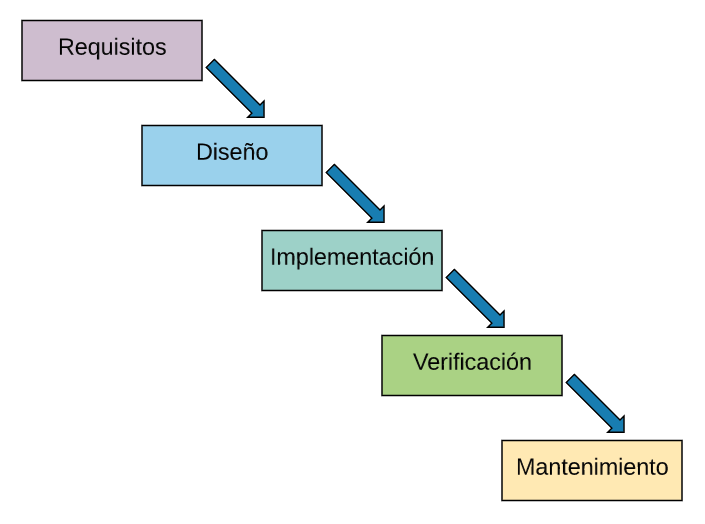
\includegraphics[width=100mm]{img/objetivos/cascada.png}
    \caption{Esquema Metodología Cascada}
\end{figure}

Como parte de la metodología, durante el tiempo que ha durado el proyecto se acordaron reuniones semanales con el tutor de forma presenciales o por Vídeo-Conferencia en las que se revisaban los objetivos semanales y se definían los nuevos hitos. Se ha mantenido también una bitácora describiendo los progresos durante el desarrollo de este TFG \footnote{\url{https://jderobot.org/Graylinx-tfg}}.

También debemos destacar en la metodología el uso de Git como infraestructura de control de versiones de software. El código desarrollado está disponible públicamente en GitHub \footnote{\url{https://github.com/RoboticsURJC-students/2016-tfg-Mario-Fernandez}}. Git es un sistema de control de versiones de código libre y abierto, el cuál esta diseñado para controlar cualquier tipo de proyectos independientemente de su magnitud.

Git mantiene todos los \textit{commit} que hagamos de nuestro proyecto. Un \textit{commit} es una foto de nuestros archivos en un determinado momento. Estos incluyen un identificador, todos los cambios respecto al \textit{commit} anterior y una referencia al mismo. De esta manera, siempre que queramos, podremos retroceder hasta una versión anterior de nuestro código.
Por otro lado, permite tener varias versiones en paralelo o ramas de nuestros proyectos. Éstas son muy útiles para trabajos en equipo, ya que cada desarrollador puede implementar sus funcionalidades en una rama \textit{branch} y luego fusionarse con \textit{(merge)} del resto.

\section{Plan de trabajo}

Para la realización de todo el proyecto se ha seguido un plan de trabajo en cinco diferentes fases:

\begin{itemize}

\item \textbf {Primera fase}: Es una fase de iniciación cuyo objetivo principal es el de aprender todo lo que tenga que ver con el desarrollo web. En esta fase deberíamos dejar conceptos básicos aclarados y empezar a manejar alguna herramienta de control de versiones como Git. Es muy recomendable en esta primera fase empezar a manejar los lenguajes de programación que quieras utilizar en el futuro.

\item \textbf {Segunda fase}: Una vez que tenemos cierta destreza con el desarrollo, empezamos a enfocar nuestra aplicación decidiendo qué tecnologías son las que mejor van a venir para nuestro modelo de aplicación. Esta fase es vital para la continuación del proyecto, ya que la mala elección de una tecnología nos puede llevar mucho tiempo.

\item \textbf {Tercera fase}: Una vez que tenemos claro qué tecnologías vamos a utilizar en nuestra aplicación, comenzamos con un sencillo prototipo que utilice todas las tecnologías que estarán implicadas en nuestra aplicación. Esto nos servirá para tener una sencilla estructura de lo que queremos montar.

\item \textbf {Cuarta fase}: Cuando tengamos claros los conceptos, manejemos los lenguajes de programación necesarios y tengamos montado un sencillo prototipo con las tecnologías que hemos seleccionado para nuestro proyecto, es momento de dar forma a nuestras ideas, extendiendo ese prototipo y aumentando las funcionalidades programadas, es decir desarrollando la aplicación en sí misma.

\item \textbf {Quinta fase}: Cuando tengamos nuestra aplicación completamente desarrollada y haciendo lo que nosotros queremos, es el momento de subirla a alguna plataforma de computación en la nube.
\end{itemize}

\chapter{Diseño e implementación}

En este capítulo describiremos en profundidad la implementación de la aplicación de gestión de clases particulares, tanto su lado cliente como su lado servidor, realizada en el proyecto. Antes, comenzaremos con el diseño del mismo para tener una visión más global y poder entender las partes constituyentes por separado.

\section{Diseño}

La aplicación que hemos desarrollado se divide en 4 grandes bloques: Node, MongoDB, Express y Angular. Cada uno de ellos se encarga de realizar una función dentro de la aplicación.

Antes de profundizar en cada bloque, todos los proyectos que utiliza la pila MEAN, siguen una estructura similar a la de la figura \ref{img:EstructuraMean}

\begin{figure}[!h]
    \centering
    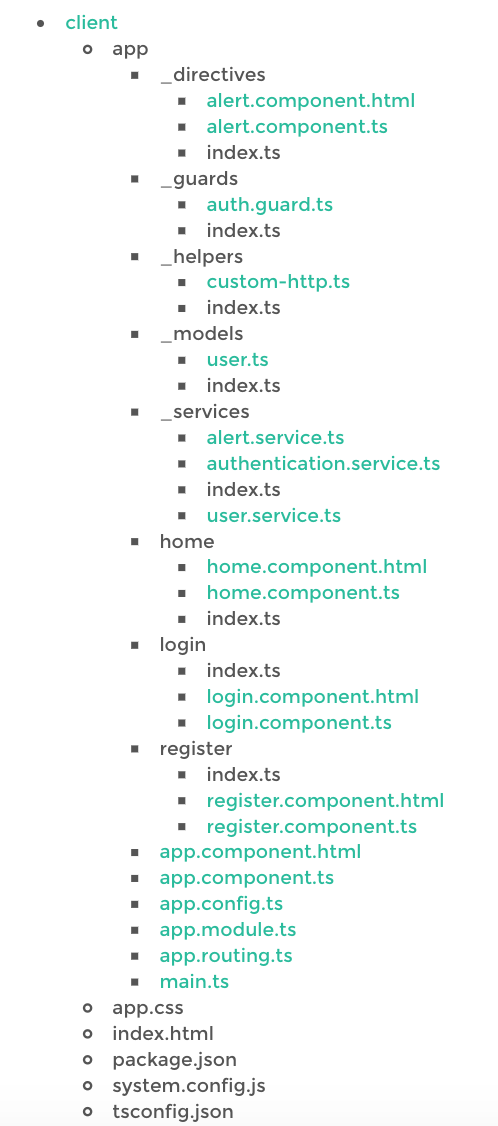
\includegraphics[width=40mm]{img/aplicacion/cliente.png}
    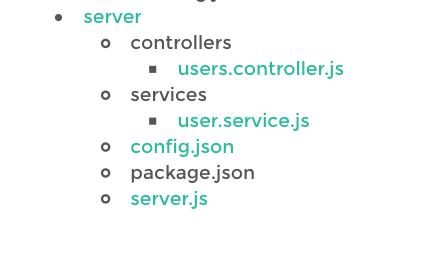
\includegraphics[width=40mm]{img/aplicacion/server.png}
    \caption{Estructura de un proyecto con la pila MEAN}
    \label{img:EstructuraMean}
\end{figure}
\section{Lado cliente de la aplicación web}

De los 8 bloques principales de una app en Angular, vamos a ir identificando uno a uno y que uso se le da en nuestra aplicación.

\subsection{Modulos: } Como las aplicaciones en Angular son modulares y un módulo es el conjunto de código dedicado a cumplir un único objetivo, los módulos utilizados en nuestra aplicación son:
\begin{itemize}
\item \textbf{NgModule from '@angular/core'} Es el módulo principal, el cual recibe un objeto que define el módulo. Los metadatos más importantes de un NgModule son:

\begin{enumerate}
\item{Declarations: } Las vistas que pertenecen a tu módulo. Hay 3 tipos de clases de tipo vista: componentes, directivas y pipes.
\item{Exports: } Conjunto de declaraciones que deben ser accesibles para plantillas de componentes de otros módulos.

\item{Imports: } Otros NgModules, cuyas clases exportadas son requeridas por templates de componentes de este módulo.

\item{Providers: } Los servicios que necesita este módulo y que estarán disponibles para toda la aplicación.

\item{Bootstrap: }: Define la vista raíz. Utilizado sólo por el root module.
\end{enumerate}

\item \textbf{RouterModule from '@angular/router'} es uno de los módulos más importantes de Angular, se encuentra dentro de la librería @angular/route, gracias a él cada vez que cambiemos de direccion URL cambiaremos de página sin necesidad de tener que interactuar con el servidor.

\item \textbf{ HttpModule, Http, RequestOptions from '@angular/http'} Otro módulo imprescindible en una aplicación Angular, se encuentra dentro de la librería @angular/http. Gracias a este módulo podemos hacer cualquier petición AJAX sin apenas tener que escribir código.

\item \textbf{ FormsModule from '@angular/forms'} Módulo encargado de añadir formularios personalizados.

\item \textbf{FileUploadModule from 'ng2-file-upload'} Es el módulo que nos permite subir imágenes y enviarlas a nuestro servidor, para luego poder almacenarlas de forma ordenada en nuestra base de datos.

\item \textbf{AgmCoreModule from 'angular2-google-maps/core} Gracias a este módulo, podemos utilizar la API de google maps en nuestra aplicación.

\item \textbf{ BrowserModule from '@angular/platform-browser'} Este módulo es necesario en cualquier app que se renderice en el navegador.


\item \textbf{ AuthGuard from './common/auth.guard'} Gracias a este modulo, podemos conservar las credenciales de un usuario durante un tiempo determinado en el navegador.

\item \textbf{ ProvideAuth, AuthHttp, AuthConfig from 'angular2-jwt'} Este módulo proporciona seguridad a nuestra aplicación, generando un \textit{token} encriptado para cada usuario que se registre en nuestra aplicación.

\item \textbf{AppComponent, Intro, LoginAlumno, LoginProfesor , HomeAlumno, HomeProfesor, SignupAlumno, SignupProfesor, ProfesorDetail } Estos son los módulos propios se han desarrollado para la aplicación de este TFG.
\end{itemize}
\subsection{Componentes: }

Los componentes son como etiquetas nuevas que podemos inventarnos para realizar las funciones que sean necesarias para nuestra aplicación de gestión de clases particulares.

Se compone de 1 componente principal y 8 componentes que derivan de él. AppComponent es el componente principal y tiene la siguiente apariencia:

\begin{lstlisting}[caption=AppsComponent]
import { Component } from '@angular/core';

@Component({
  selector: 'app-root',
  templateUrl: './app.component.html',
  styleUrls: ['./app.component.css']
})
export class AppComponent {
  title = 'ClassCity';
}
\end{lstlisting}

El selector app-root o el nombre de la etiqueta que se usará cuando se desee representar. Con la propiedad templateUrl asociamos un archivo .html que se usará como vista del componente. Por último se define su estilo mediante la propiedad StyleUrls, indicando a un array de todas las hojas de estilos que deseamos.

\subsubsection{Componentes secundarios }

\begin{itemize}
\item \textbf{Intro} Este componente corresponde con la página introductoria a la aplicación donde podemos elegir entre qué perfil de usuario queremos adoptar: Profesor o Alumno. Como podemos ver en la figura \ref{img:introclasscity}.

\item \textbf{LoginAlumno, LoginProfesor} Componentes encargados de realizar la función de login del alumno o del profesor como podemos ver en las figuras \ref{img:loginalumnoclasscity} \ref{img:loginprofesorclasscity}. Hemos desarrollado una función que se encarga de realizar una petición POST al servidor. Si la respuesta es aceptada, el alumno accedera a la aplicación y se almacenarán las credenciales en el \textit{localstorage} del navegador con un tiempo de caducidad de 1 hora. Mientras que si la petición es rechazada, el servidor nos enviará un mensaje avisando de que \textit{The username or password don't match}.

\item \textbf{SignupAlumno, SignupProfesor} Estos componentes se van a encargar de registrar a profesores y alumnos en nuestra base de datos. Para ellos hemos desarrollado una función en cada componente que simplemente se encarga de enviar al servidor una petición POST con un cuerpo donde se encuentran los datos personales del profesor o el alumno. Figura \ref{img:signupalumnoclasscity} \ref{img:signuprofesorclasscity}

\item \textbf{HomeAlumno, HomeProfesor} Cuando un profesor o un alumno es aceptado dentro de nuestra base de datos y consigue entrar en la aplicación, puede realizar diferentes funciones dependiendo de si entro como alumno o como profesor. figuras \ref{img:homealumnoclasscity} \ref{img:homeprofesorclasscity}.

\begin{enumerate}
\item \textbf{Alumno }  Un alumno puede realizar la búsqueda del profesor que más le interese por diferentes parámetros:
\begin{itemize}
    \item{El curso en el que está el alumno}
    \item{La asignatura que quiere cursar}
    \item{La distancia a la que se encuentre el profesor}
\end{itemize}

\item \textbf{Profesor } La página del profesor consiste en un chat realizado con \textit{websockets}, donde podrá entablar conversación con cualquier alumno que este interesado en él. Aparte puede personalizar su perfil, cambiando la foto que tiene como avatar.
\end{enumerate}

\item \textbf{ProfesorDetail} Cuando un alumno encuentra a su profesor particular ideal desde la página del alumno y hace click sobre el profesor interesado, el componente ProfesorDetail se lanza y consiste en una ficha técnica del profesor particular, así como un chat donde el alumno podrá comunicarse con el profesor para poder quedar y acordar el precio de la clase tal y como podemos ver en la figura \ref{img:detailprofesorclasscity}

\end{itemize}

\subsection{Plantilla }

Las plantillas se utilizan para dar forma a las aplicaciones. Es la parte más visual de una aplicación web y es la propia magia de Angular la que se encarga de renderizar estas plantillas, haciendo aplicaciones mucho más personalizadas para el usuario. A continuación vamos a ir analizando una a una las diferentes plantillas que forman la aplicación de gestión de clases particulares:

\textbf {intro.html} Cuando accedemos a la URL \footnote{\url{https://www.classcity.es}} de la aplicación, la primera plantilla que se nos presenta es Intro.html. Según podemos ver en la imagen  \ref{img:introclasscity}, consiste en una página introductoria donde podemos elegir si somos alumnos o porfesores.

\begin{figure}[!h]
    \centering
    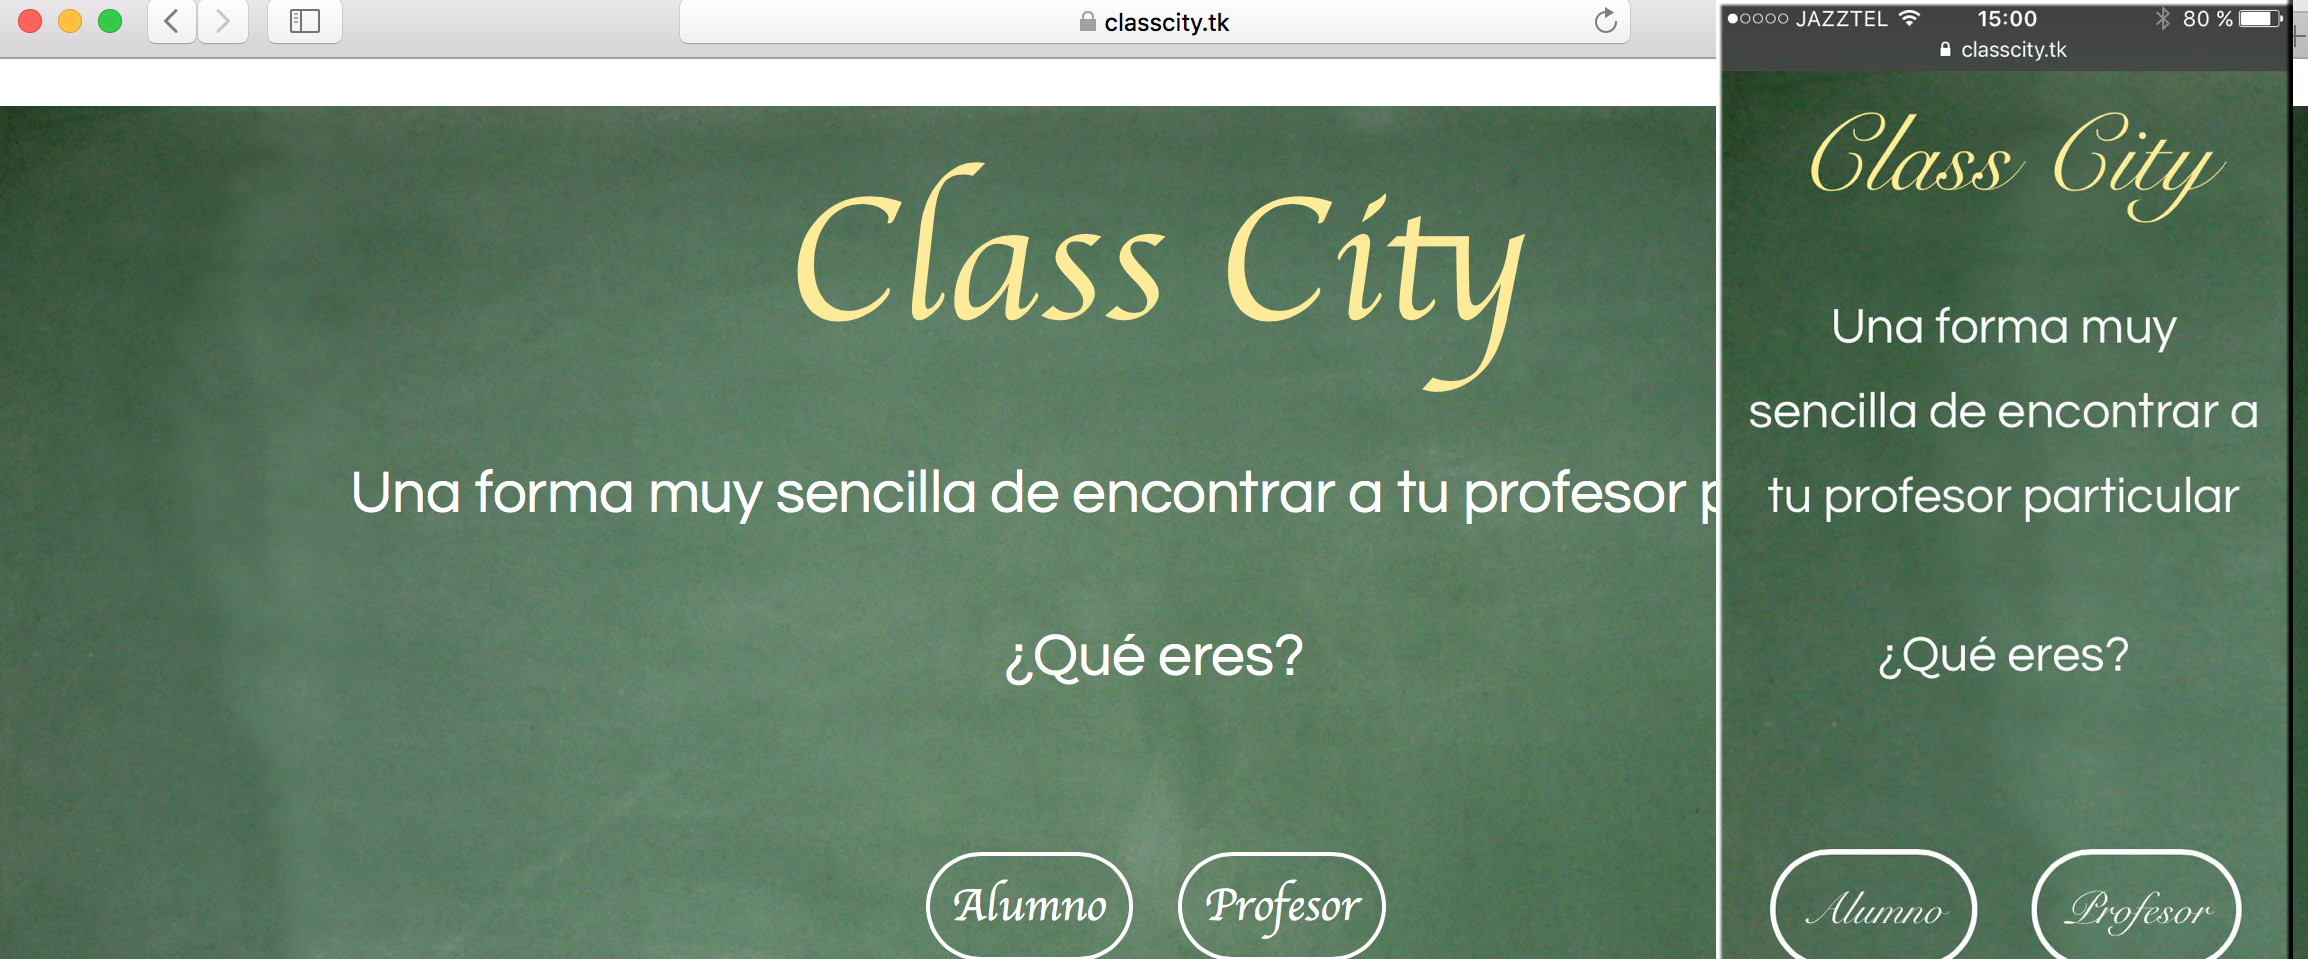
\includegraphics[width=140mm]{img/templates/intro.png}
    \caption{Página Intro ClassCity}
    \label{img:introclasscity}
\end{figure}


\textbf{loginalumno.html} Al seleccionar dentro de Intro.html en Alumno, accedemos a la siguiente plantilla donde podemos visualizar un formulario con sus campos \textit{username} y \textit{password}. Además de resaltar la caracteristica resposive de la aplicación, demostrando que es totalmente adaptable para dispositivos moviles como para ordenadores.

\begin{figure}[!h]
    \centering
    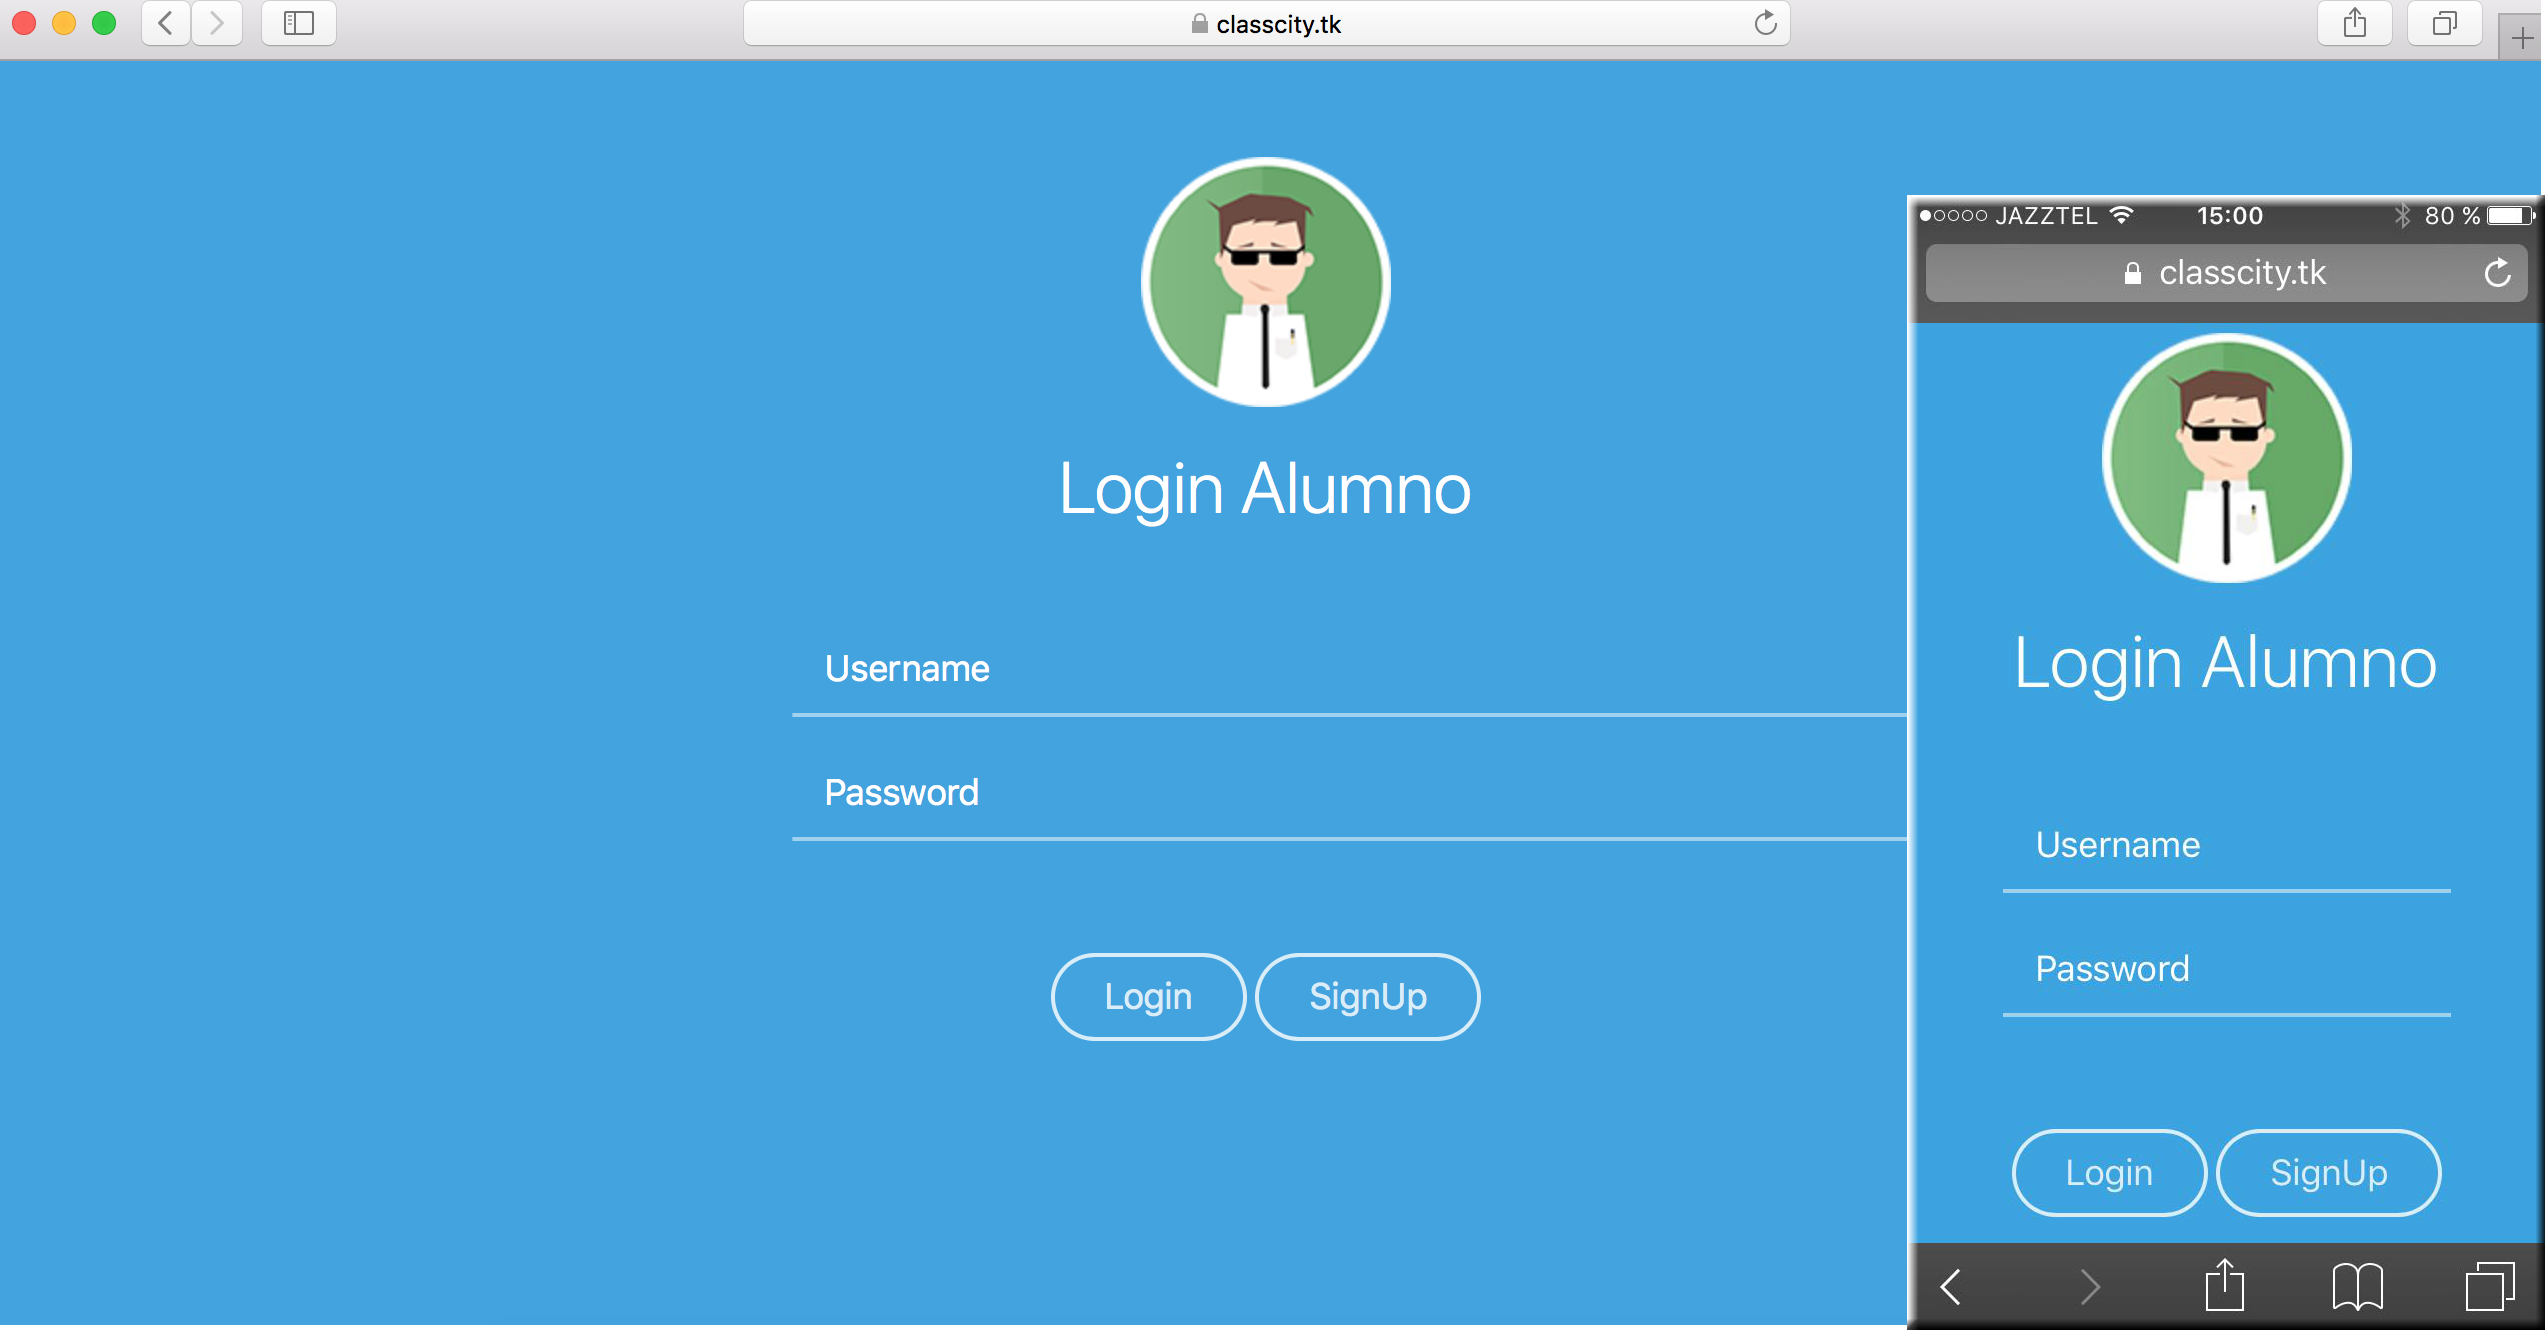
\includegraphics[width=140mm]{img/templates/loginalumno.png}
    \caption{Página Login Alumnos}
    \label{img:loginalumnoclasscity}
\end{figure}


\textbf{loginprofesor.html} Si en vez de seleccionar Alumno hubiésemos seleccionado Profesor en la página introducctoria, hubiesemos entrado en otro formulario donde los profesores ya registrados pueden acceder a la aplicación.Al igual que la plantilla de \textit{loginalumno.html} es totalmente resposive. Para poder controlar que la plantilla sea resposinve hemos utilizado diferentes ficheros css \textit{(movil.css y ordenador.css)} por cada plantilla en todas las plantillas de la aplicación.
\begin{figure}[!h]
    \centering
    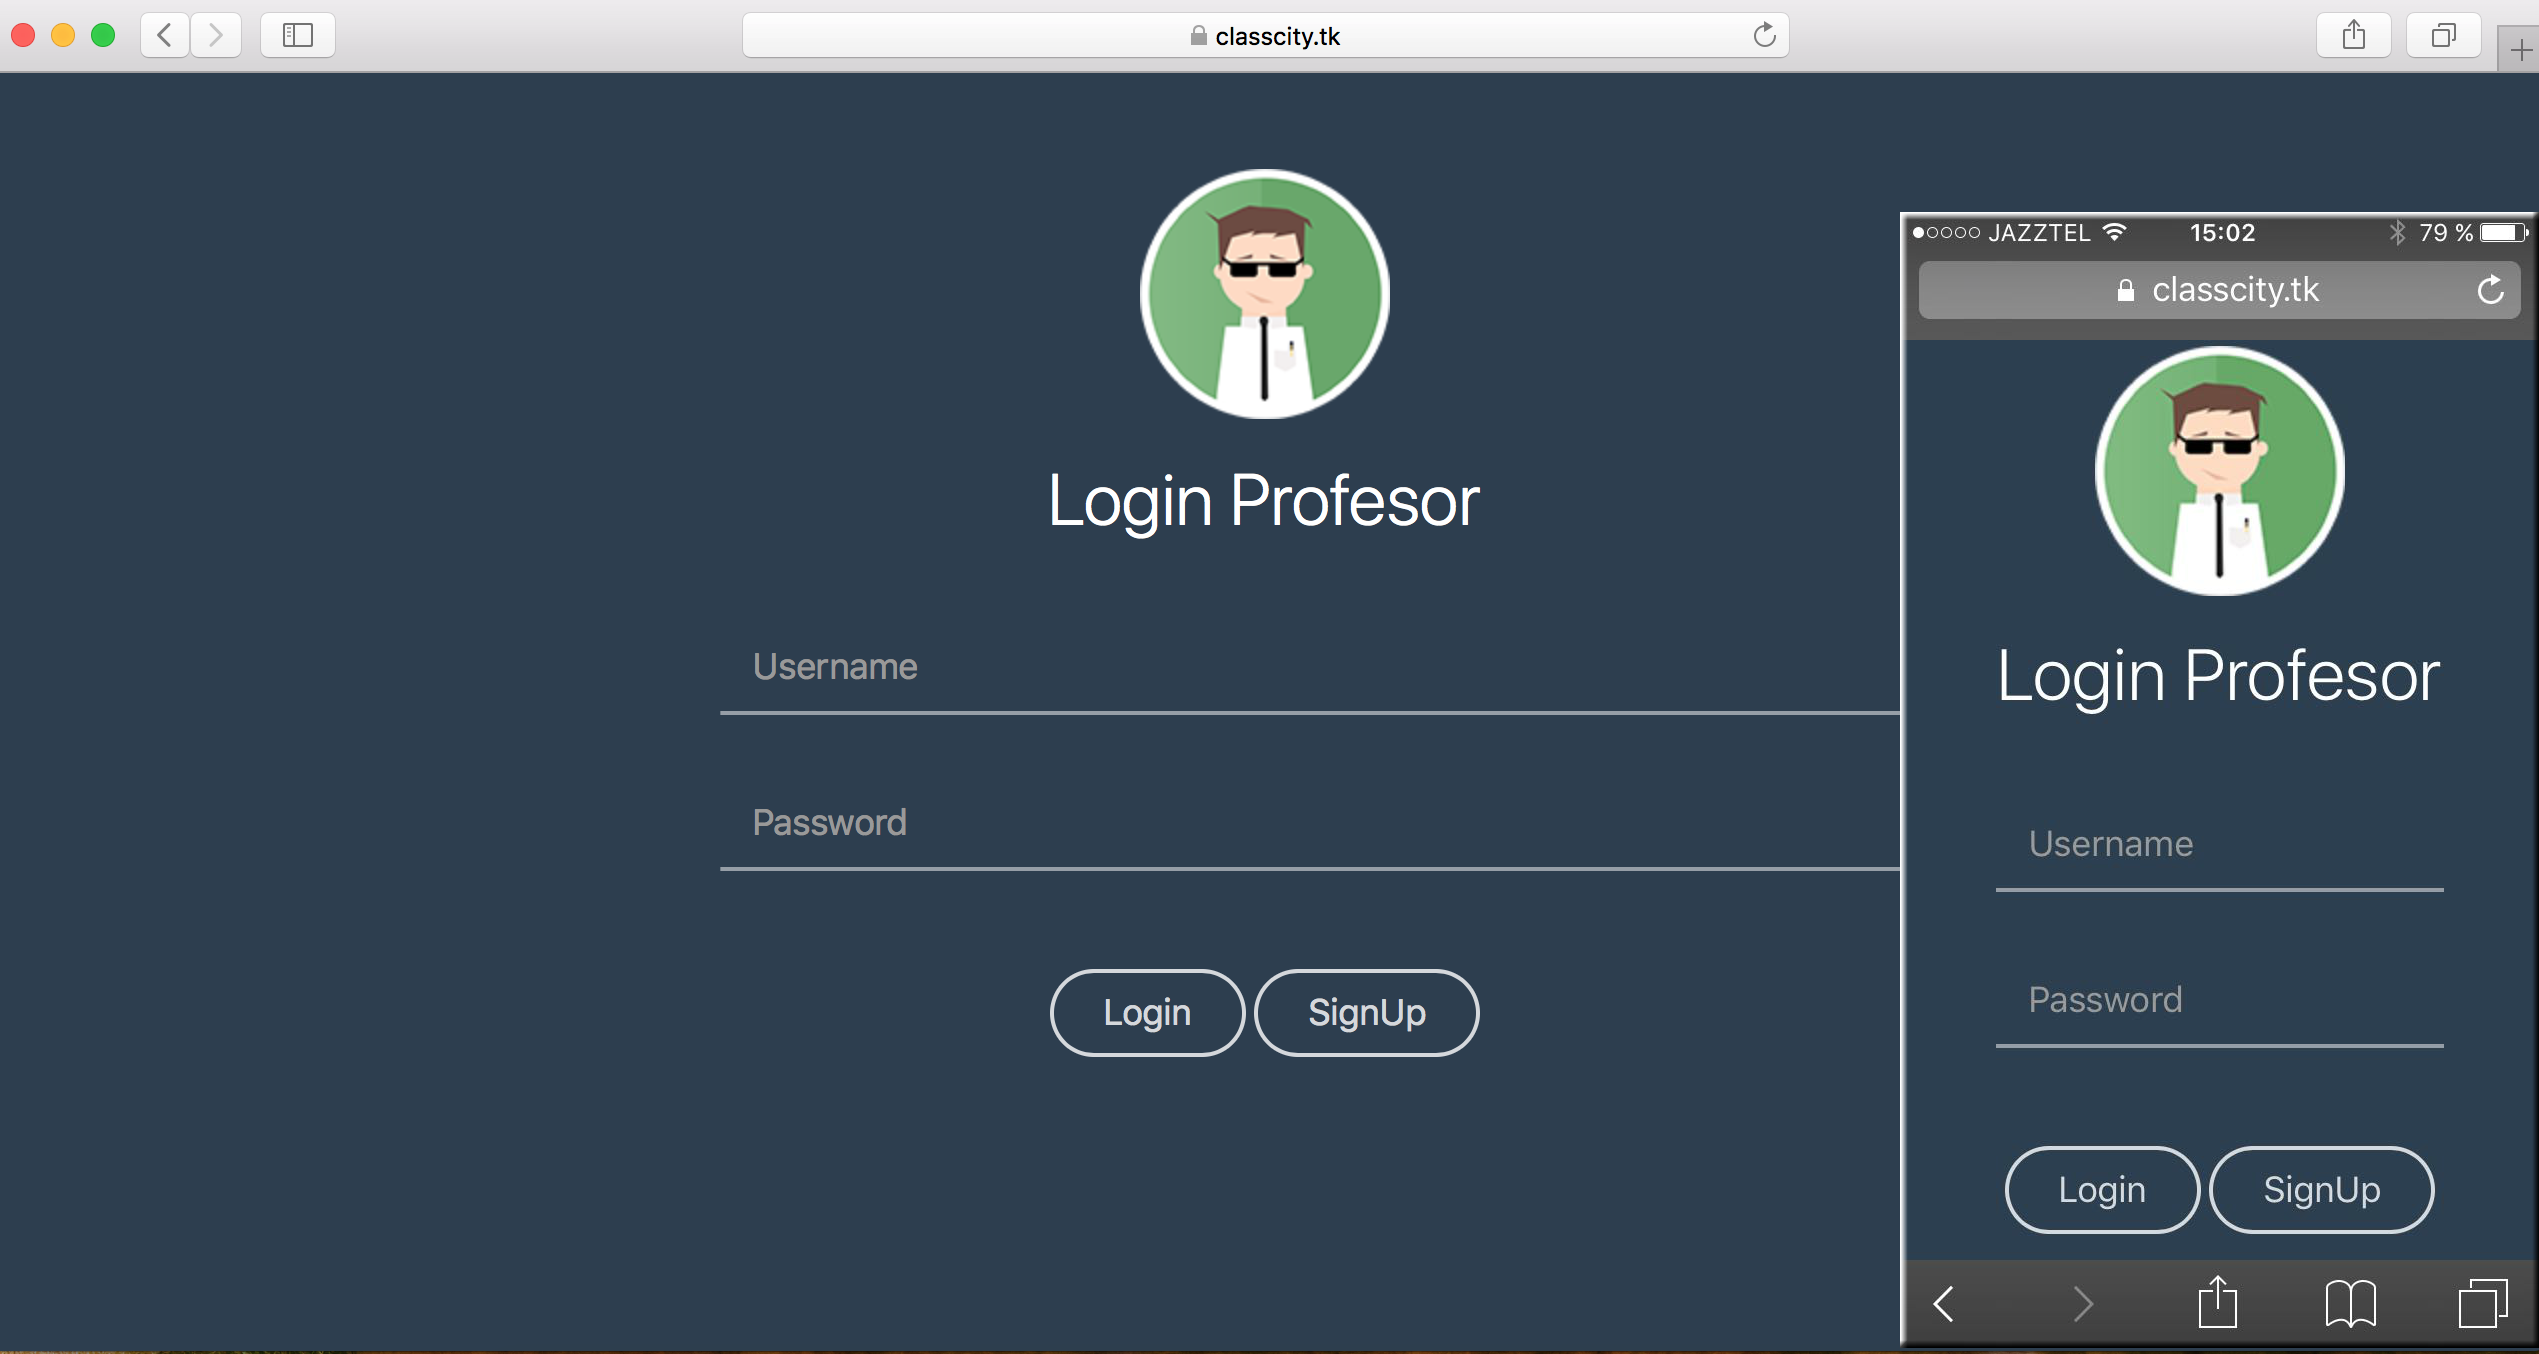
\includegraphics[width=140mm]{img/templates/loginprofesor.png}
    \caption{Página Login Profesor}
    \label{img:loginprofesorclasscity}
\end{figure}

\textbf{registeralumno.html} Si un alumno quiere registrase simplemente debe entrar en SignUp, donde tendrá un formulario para poder completar todos los campos necesarios. Los datos que solicitamos para el alumno son los siguientes: Email, Password, Nombre, Apellidos y Fecha de Nacimiento. Todos estos datos serán enviados a nuestro servidor donde almacenaremos la información.
\begin{figure}[!h]
    \centering
    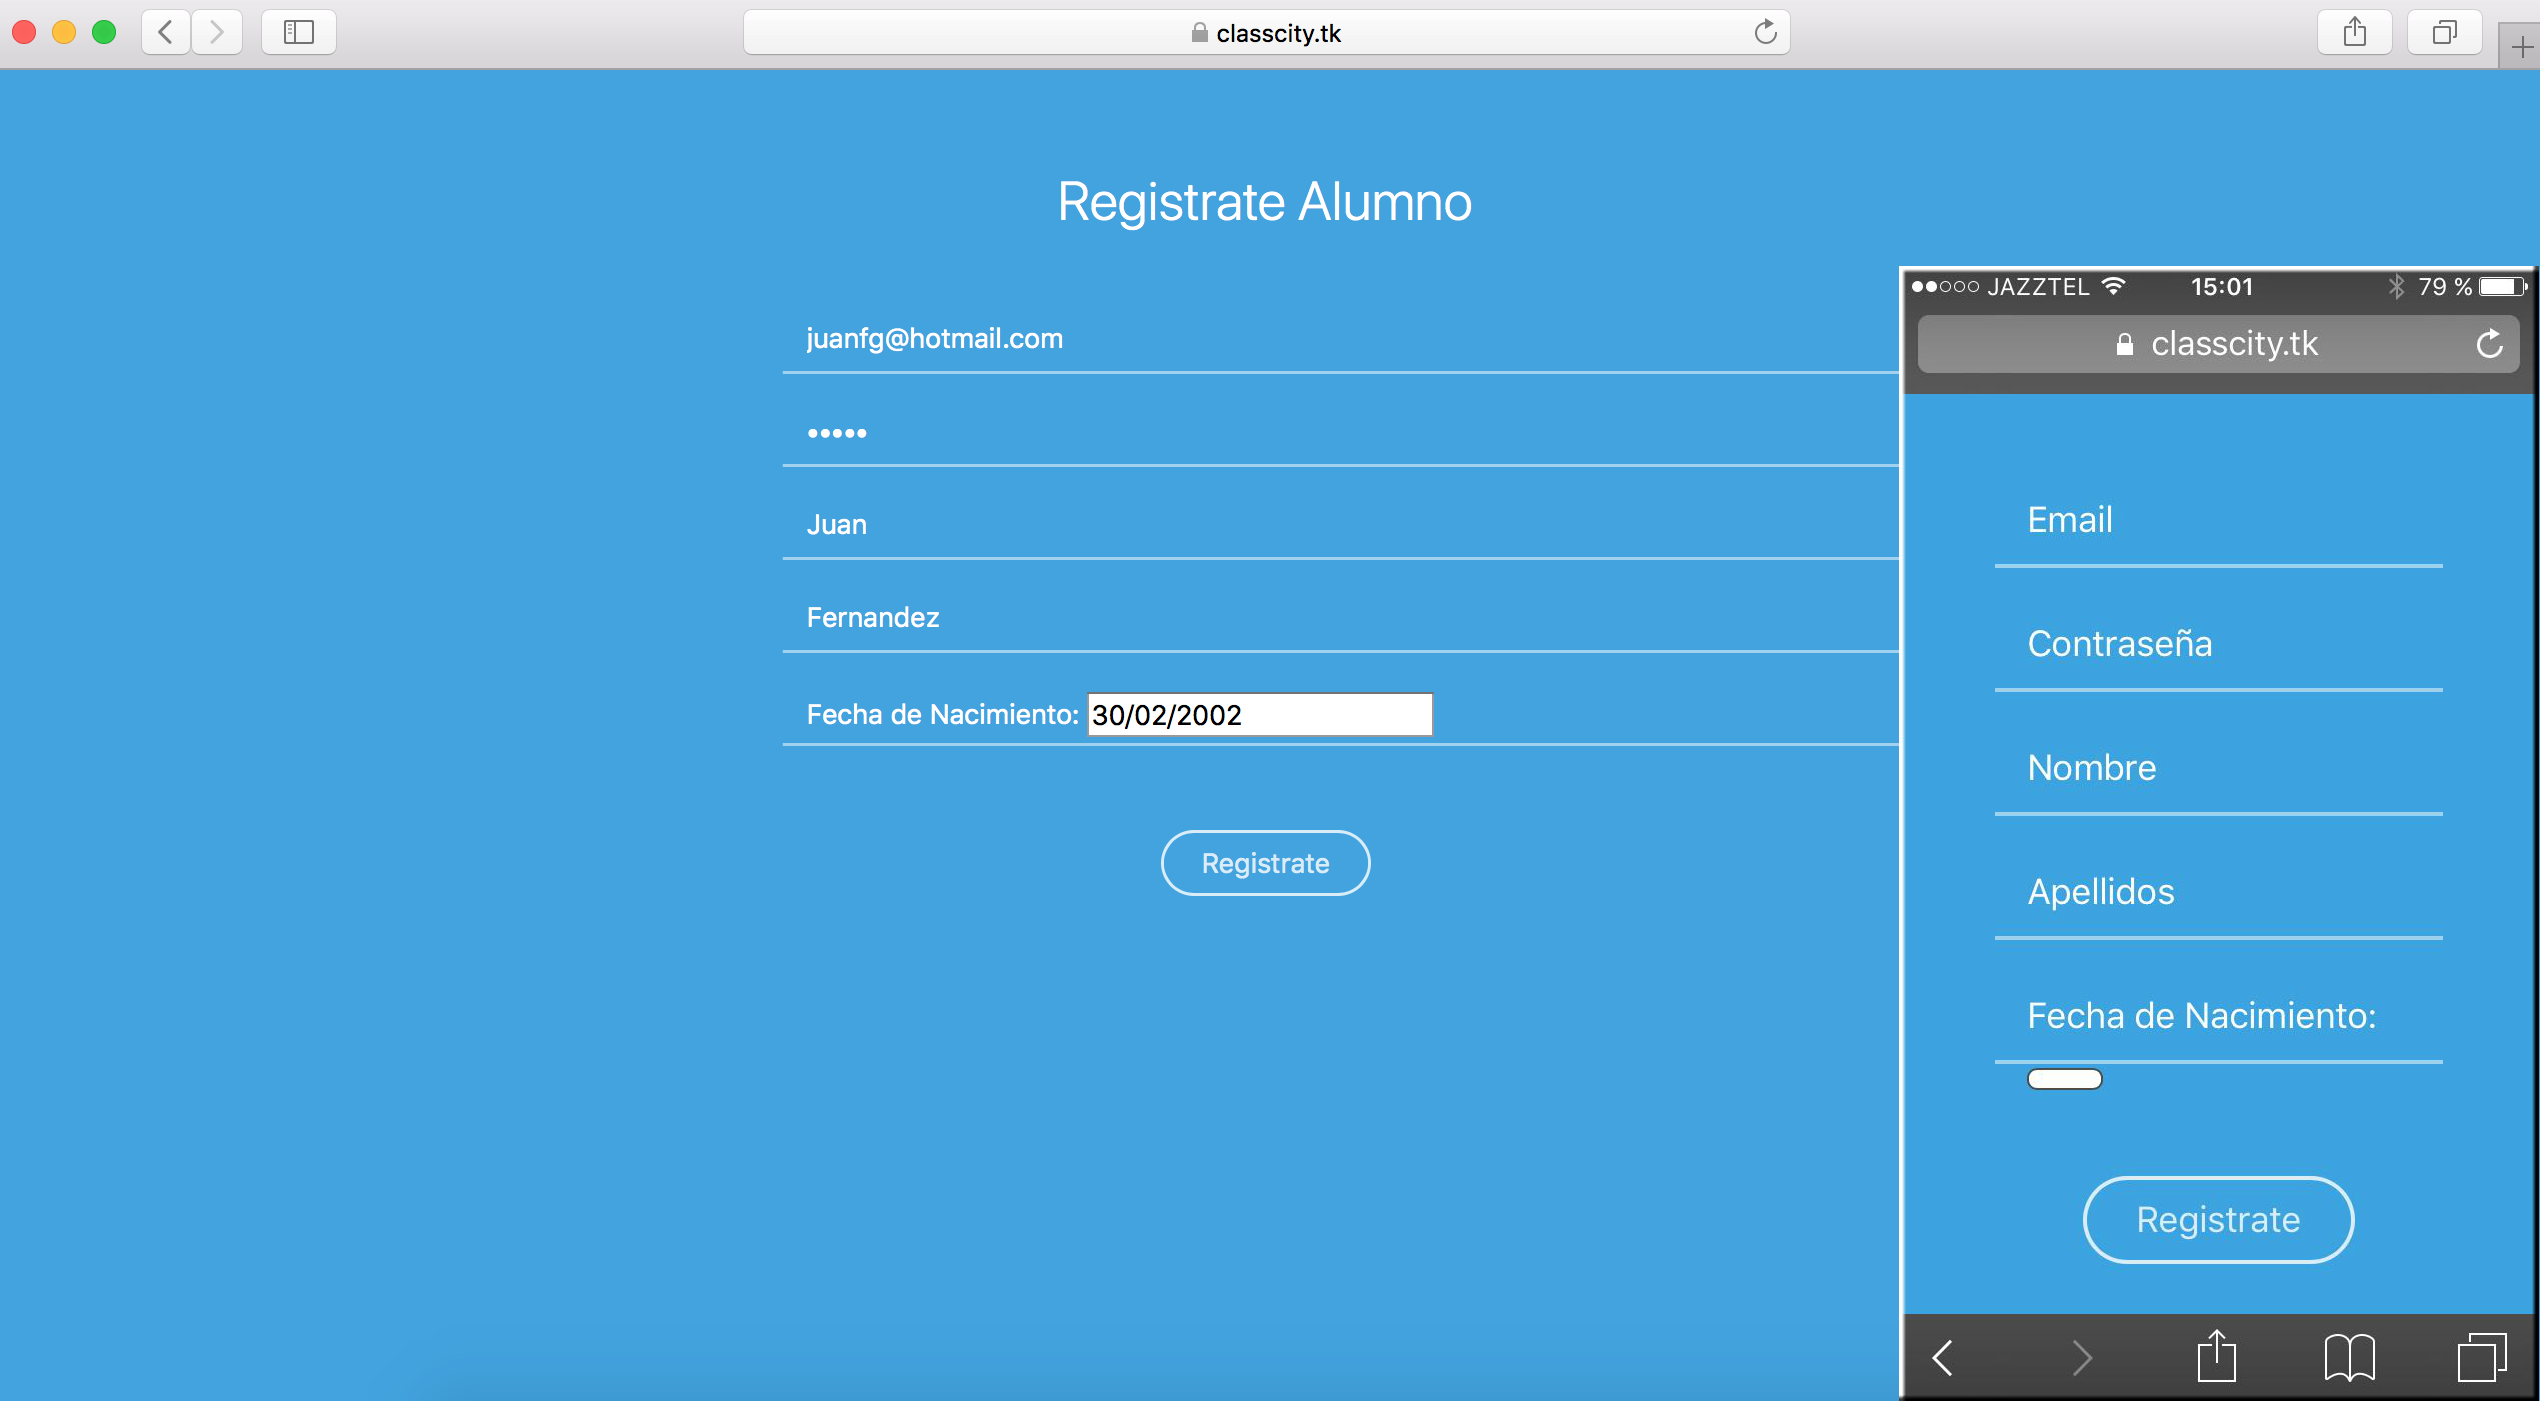
\includegraphics[width=140mm]{img/templates/registeralumno.png}
    \caption{Página Registrar Alumno}
      \label{img:signupalumnoclasscity}
\end{figure}

\textbf{registerprofesor.html} Si es el profesor quien quiere registrarse en nuestra aplicación, entrará en SignUP de profesores e introducirá los datos necesarios. Los datos que solicitamos al profesor son: Ubicación, Nombre, Apellidos, Password, Email, Fecha de Nacimiento, Curso y Asignatura.
\begin{figure}[!h]
    \centering
    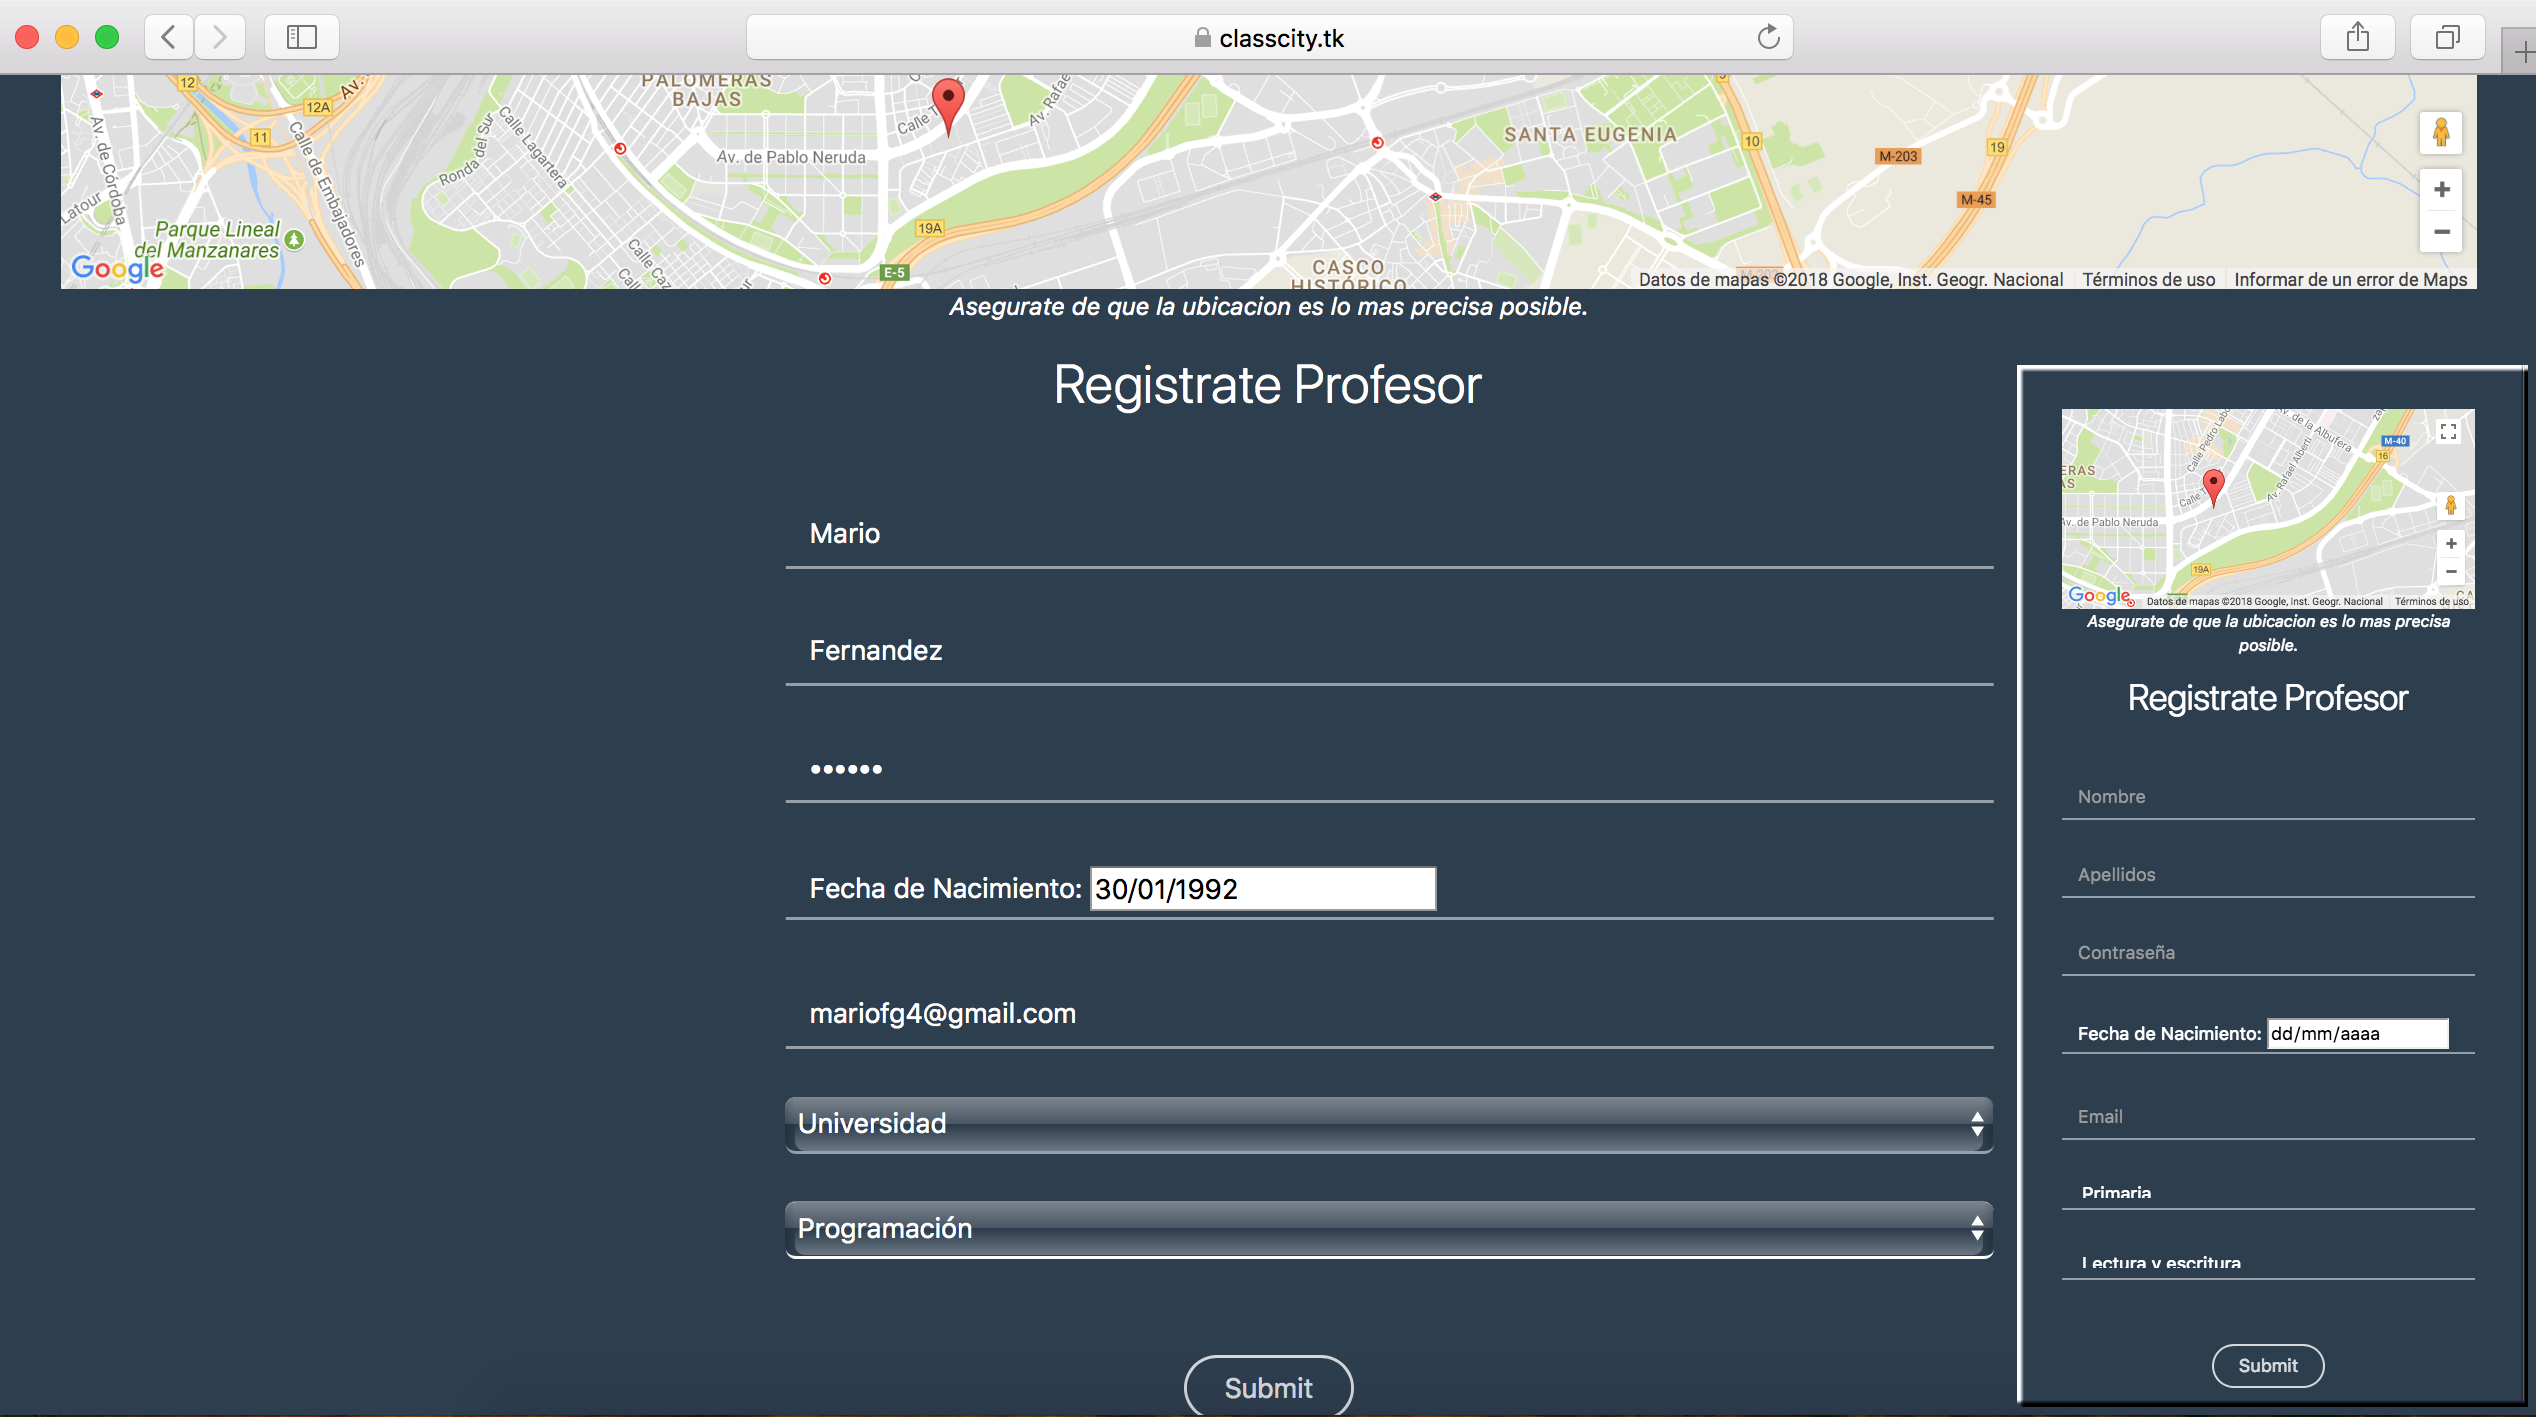
\includegraphics[width=140mm]{img/templates/registerprofesor.png}
    \caption{Página Registrar Profesor}
    \label{img:signuprofesorclasscity}
\end{figure}

\textbf{homealumno.html} Una vez que el alumno ya ha sido registrado en nuestra base de datos, la interfaz con la que se encontrará el es la que podemos ver en la figura \ref{img:homealumnoclasscity}.
Podemos apreciar una entrada en el mapa para introducir la ubicación donde queremos buscar. También podemos diferenciar los filtros de búsqueda que tenemos para buscar a nuestro profesor. Por último, cuando el alumno busca con los parámetros que desee, les aparecerán pintados en el mapa tantos profesores como haya en nuestra aplicación con esas especificaciones.
\begin{figure}[!h]
    \centering
    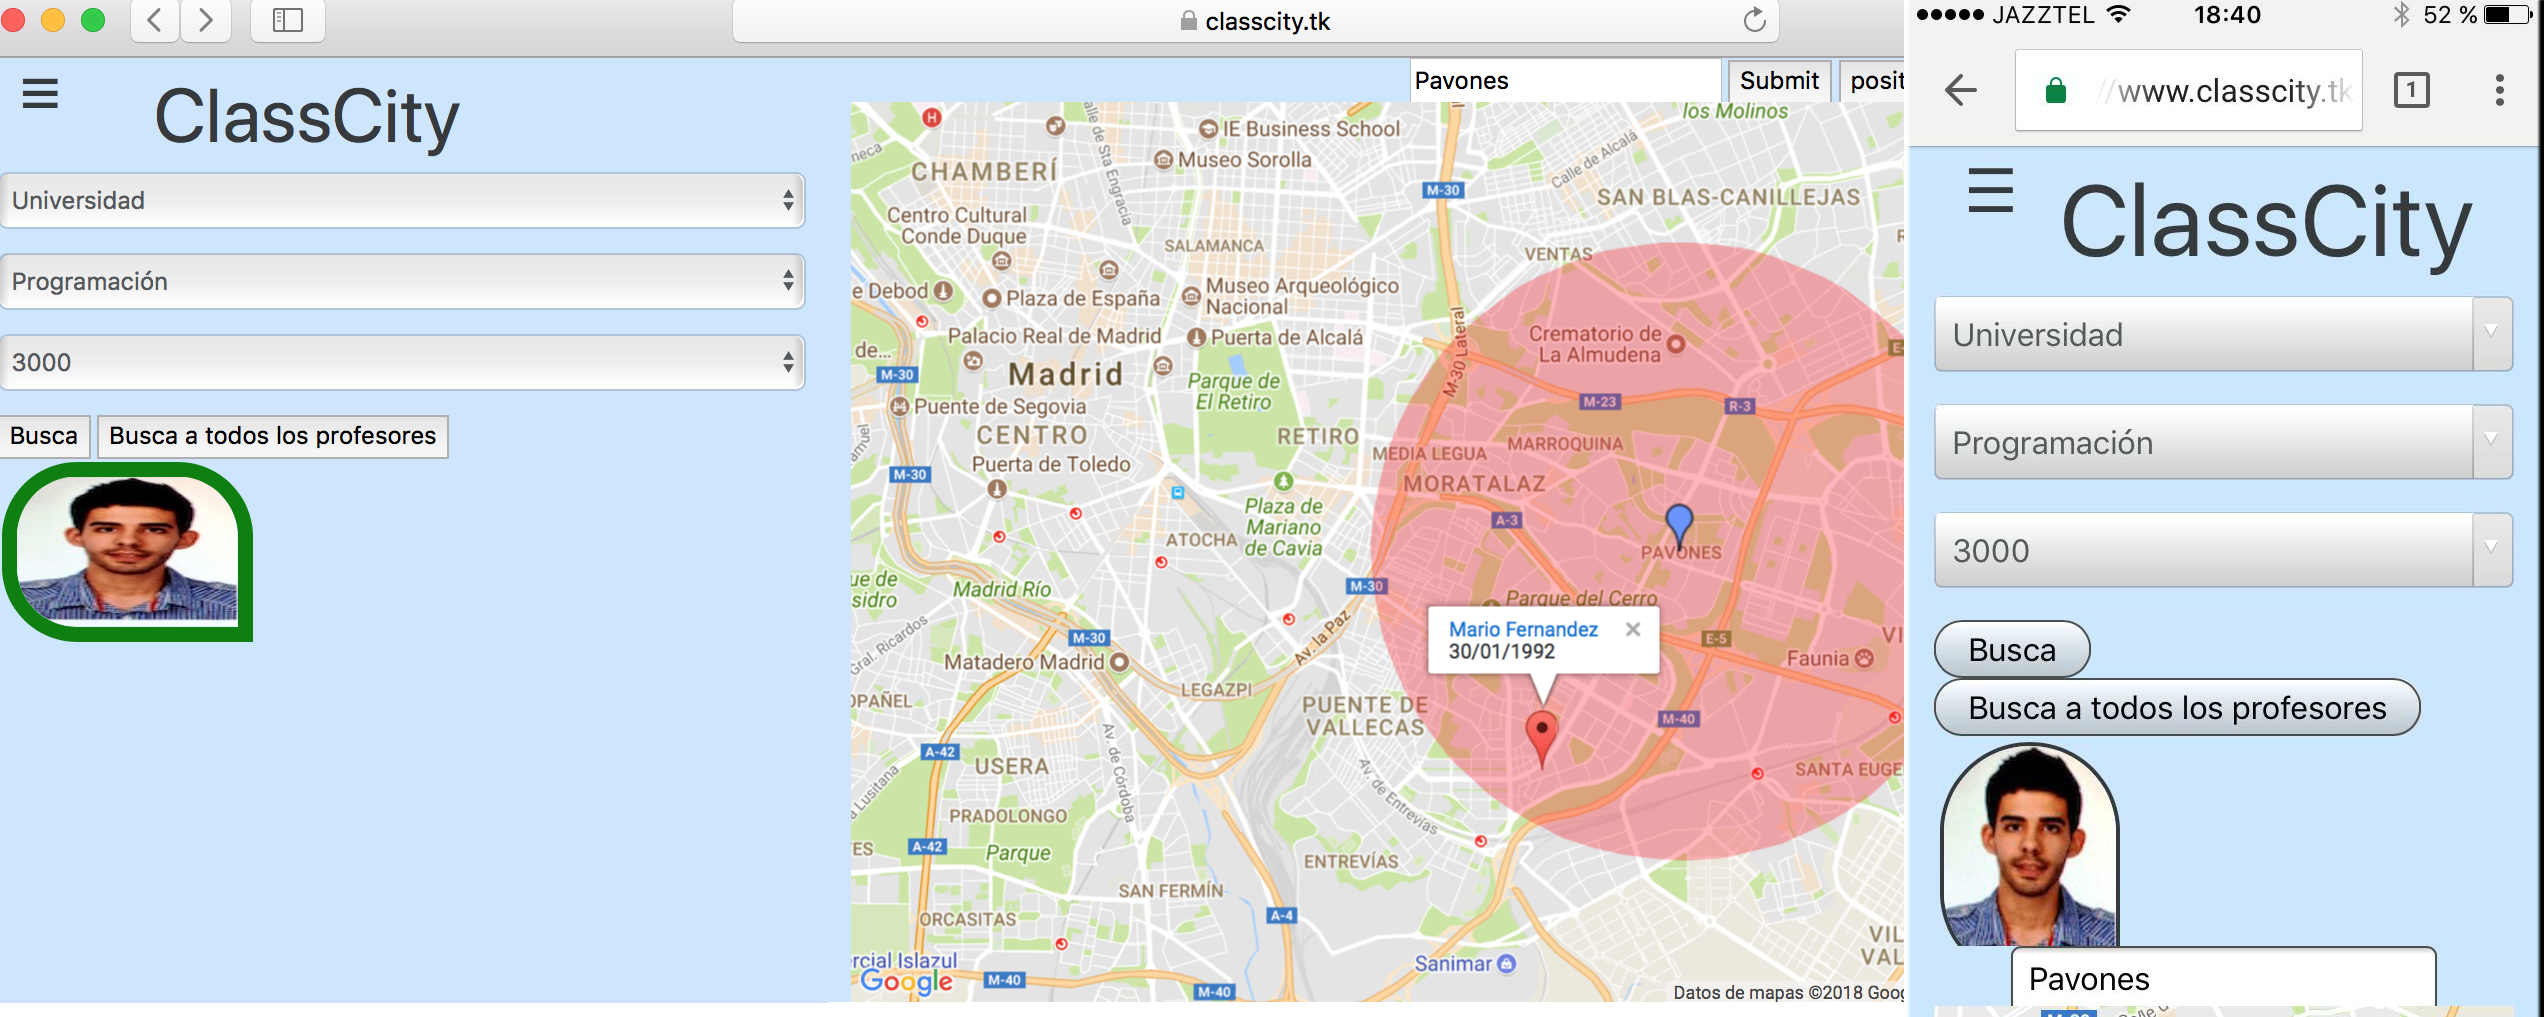
\includegraphics[width=160mm]{img/templates/homealumno.png}
    \caption{Página Home Alumno}
    \label{img:homealumnoclasscity}
\end{figure}

\textbf{detail.html} Cuando el alumno encuentra algún profesor de su interés puede hacer click sobre la imagen del profesor y así entrar en más detalle, viendo su ficha técnica y pudiendo entablar una conversación a partir del chat. La ficha técnica muestra los siguientes datos del profesor: Nombre, Apellidos, Asignatura y Curso.
\begin{figure}[!h]
    \centering
    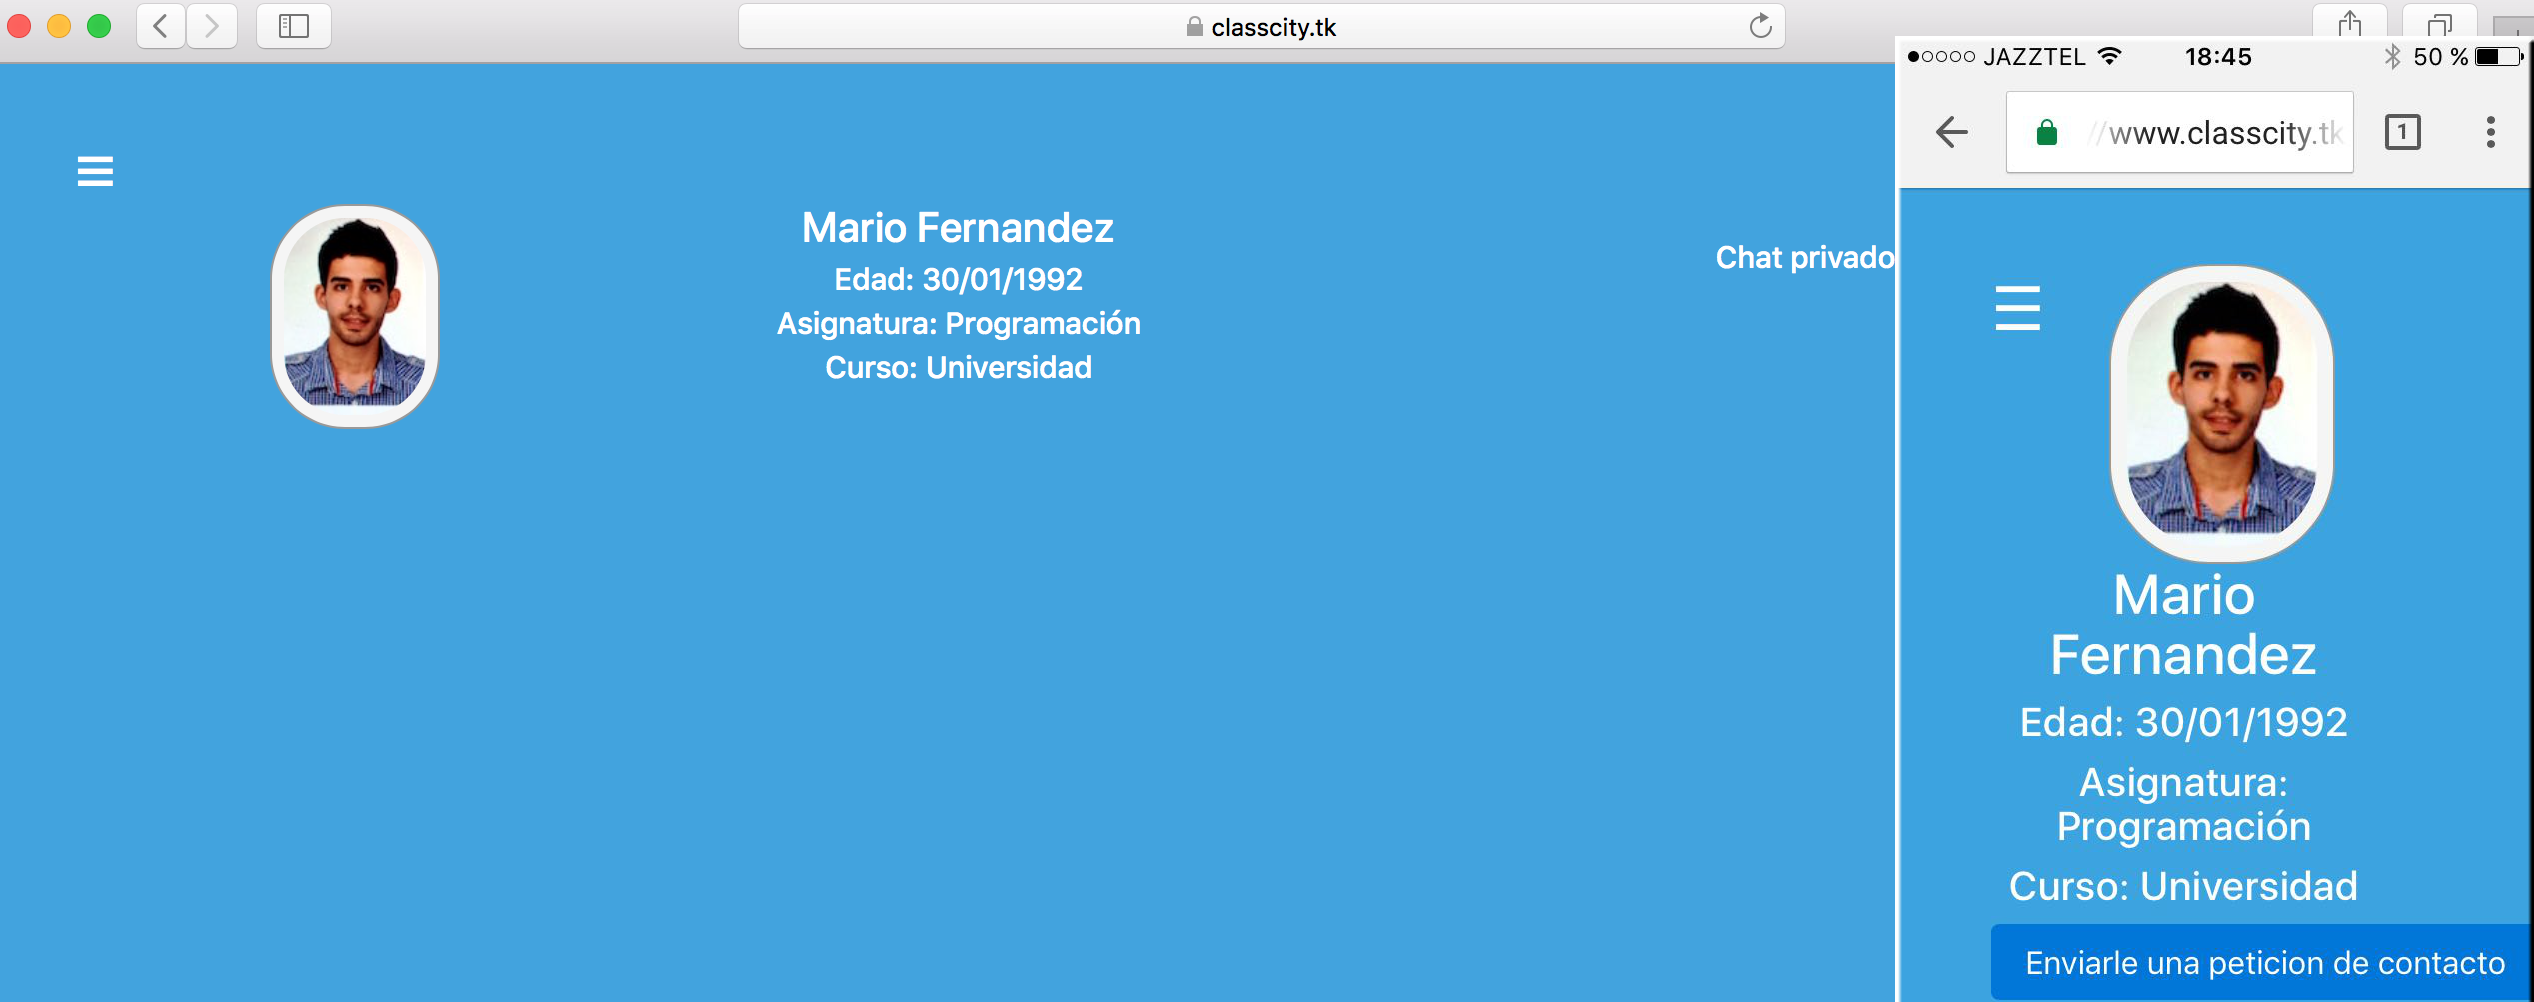
\includegraphics[width=160mm]{img/templates/detailprof.png}
    \caption{Página Detalle del Profesor}
    \label{img:detailprofesorclasscity}
\end{figure}

\textbf{homeprofesor.html} Cuando el profesor ya ha sido registrado en nuestra aplicación, el home del profesor es habilitado y en él puede hablar por un chat privado con todos los alumnos que le escriban por su canal, además de poder editar la foto de su perfil.
\begin{figure}[!h]
    \centering
    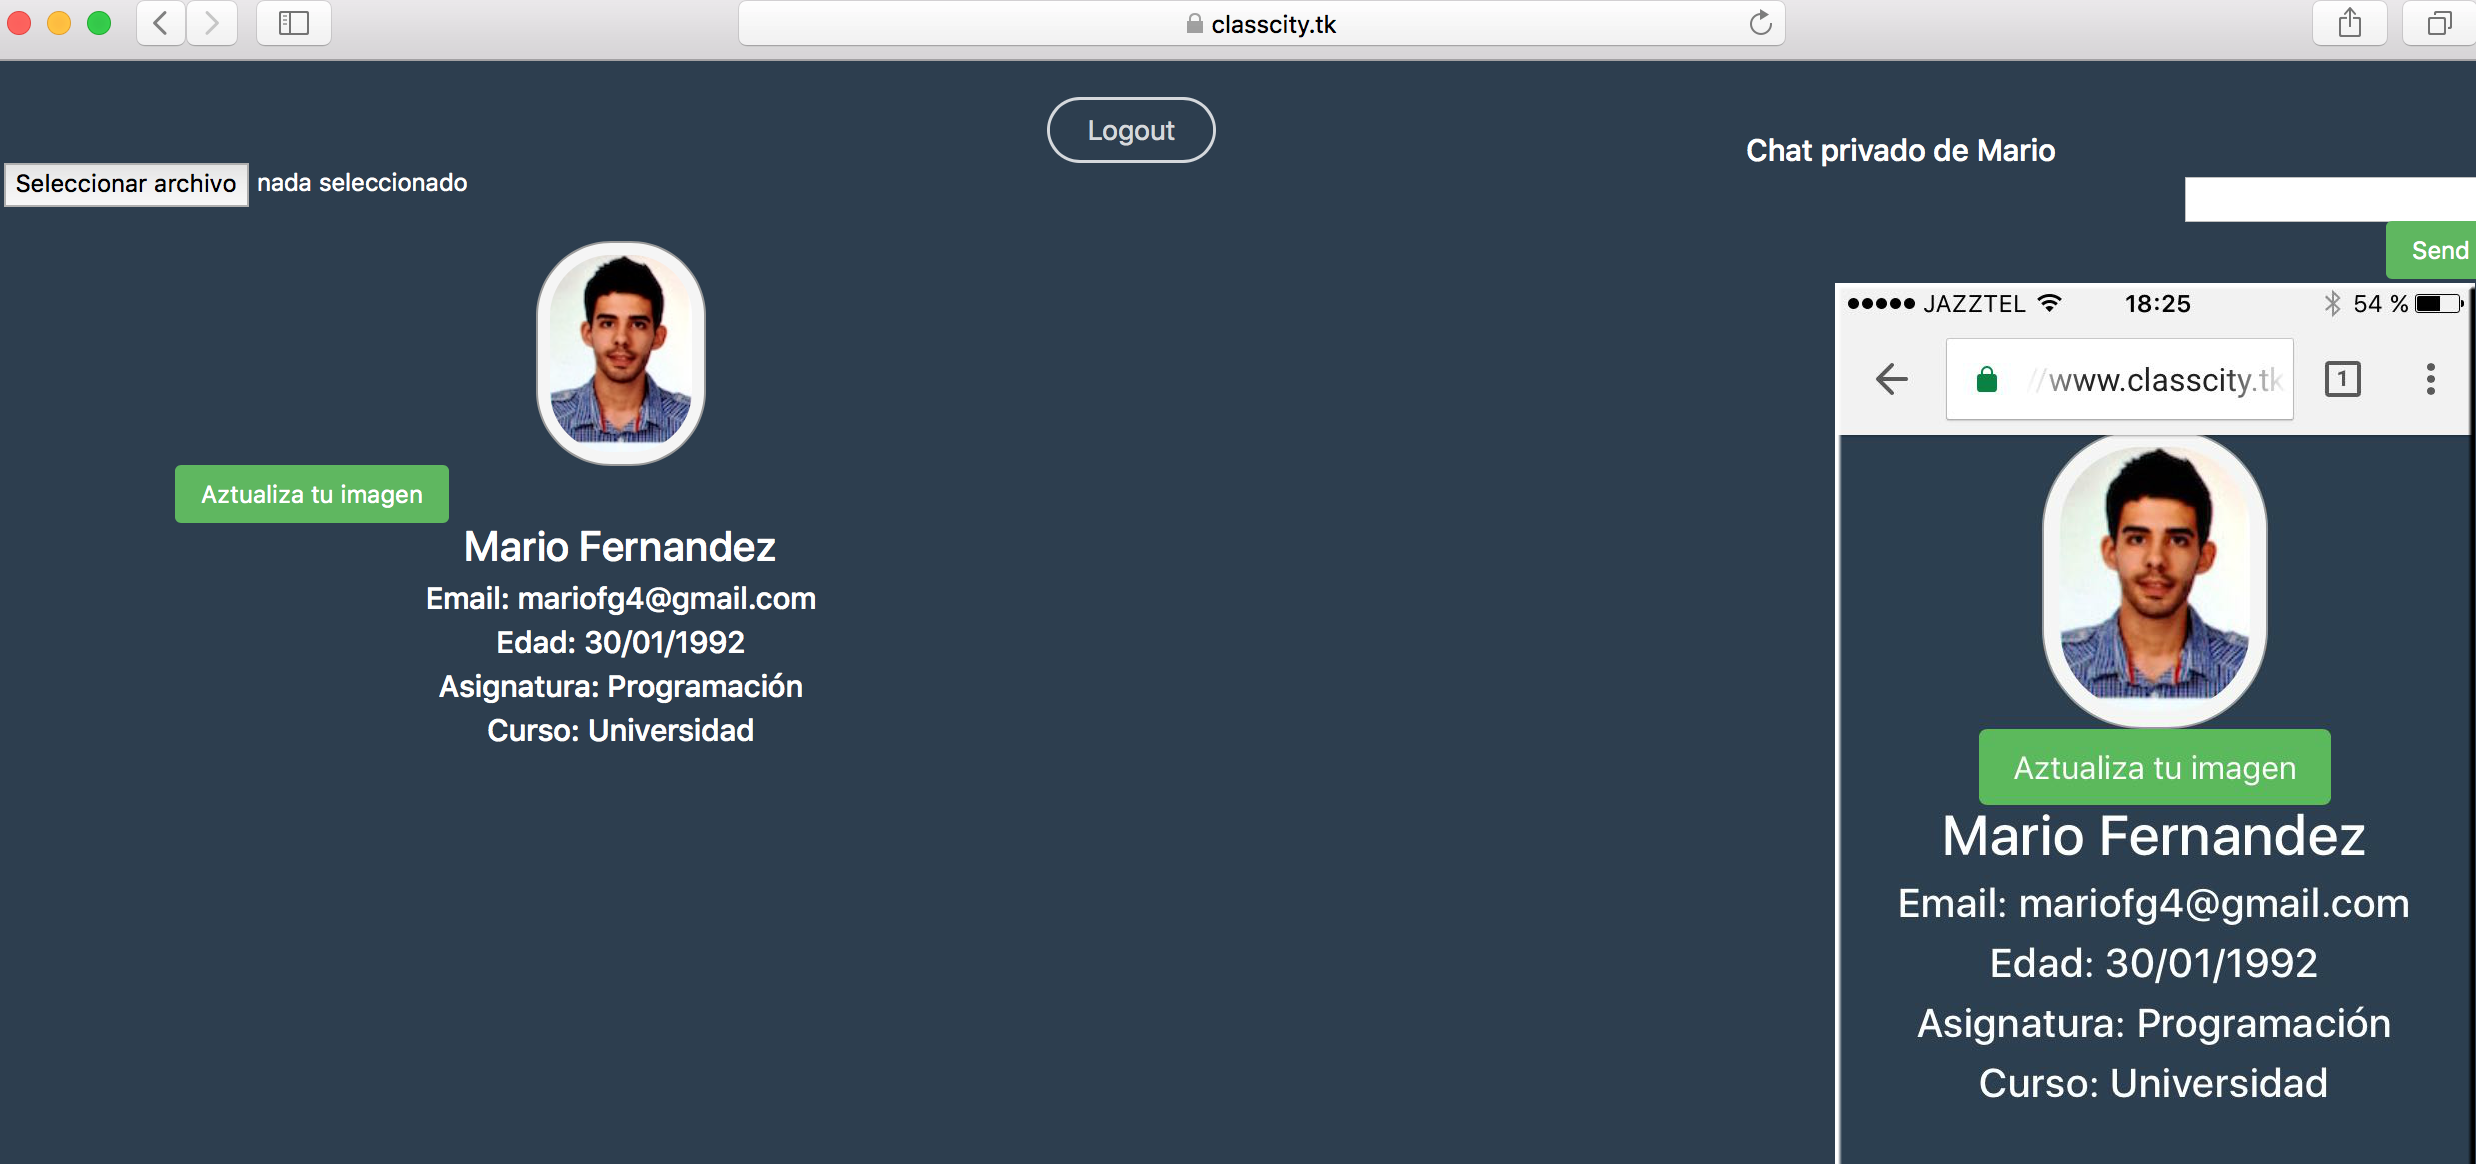
\includegraphics[width=160mm]{img/templates/homeprof.png}
    \caption{Página Home Profesor}
    \label{img:homeprofesorclasscity}
\end{figure}

\subsection{Data Binding} El Data Binding nos abstrae de la lógica \textit{pull/push} asociada a insertar y actualizar valores en el HTML y convertir las respuestas de usuario(inputs, clicks, etc) en acciones concretas.

Como se ha comentado en el capítulo anterior Angular tiene 4 formas de Data Binding, todas ellas se han utilizado en nuestra aplicación para realizar las siguientes funciones:

\textbf{Interpolación(Hacia el DOM)} Angular evaluá todas las variables e introduce su resultado en el DOM. En el siguiente ejemplo estamos insertando en el árbol DOM, todos los datos del usuario, consiguiendo una apariencia de la página mucho más personalizada.

\begin{lstlisting}
<code>{{decodedJwt.Email}}</code></pre>
<code>{{decodedJwt.id.nombre}}</code></pre>
<code>{{decodedJwt.id.apellidos}}</code></pre>
<code>{{decodedJwt.id.edad}}</code></pre>
\end{lstlisting}

\textbf{Property binding: (Hacia el DOM))} Este tipo de Data Binding, permite pasar los objetos que queramos de nuestro componente padre ('home') a la propiedad (Latitud, Longitud, radius, fillColor) del componente hijo, en este caso sebm-google-map-circle. Para ello el componente hijo tiene que tener predefinidas ciertas entradas en su directiva.

\begin{lstlisting}
<sebm-google-map-circle
    [latitude]="query.Loc.lat"
    [longitude]="query.Loc.lng"
    [radius]="query.Radio"
    [fillColor]="'red'">
</sebm-google-map-circle>
\end{lstlisting}

\textbf{Event binding: (Desde el DOM)}
Si queremos invocar a una función cuando se lance un evento, como por ejemplo cuando queremos hacer click en el botón de LogOut. En el momento que hacemos click sobre el boton de logout, la función logout es invocada y salimos de la sesión.

\begin{lstlisting}
<button type="Submit" (click)="logout()">Logout</button>
\end{lstlisting}

\textbf{Two-way binding: (Desde/Hacia el DOM)}

Cuando queremos combinar el \textit{Event Binding y el Property Binding} tenemos el binding bi-direccional, como podemos ver en el siguiente ejemplo.

\begin{lstlisting}
<input [(ngModel)]="address">
\end{lstlisting}

En este caso queremos que el valor de 'address' se actualice en el componente y que a su vez se introduzca dentro de la entrada como en el caso de \textit{property binding}.

\subsection{Directiva: }Las directivas son como los componentes, pero sin una plantilla asociada. En nuestro caso hemos utilizado directivas para realizar varias funciones, por ejemplo:

\textbf{FileSelectDirective, FileDropDirective, FileUploader} Estas tres directivas proceden del módulo "FileUploadModule", y sirven para poder subir una imagen desde el escritorio local del usuario al navegador, para luego enviar la imagen al servidor.

\begin{lstlisting}
<input type="file" ng2FileSelect [uploader]="uploader" />
\end{lstlisting}
\textbf{sebm-google-map, sebm-google-map-marker} Estas son otras de las directivas procedentes del módulo 'agmCoreModule', el cual nos proporciona toda la interfaz de programación de GoogleMaps. Gracias a estas directivas podemos jugar con el API de google en nuestra aplicación angular.

\begin{lstlisting}
<sebm-google-map *ngIf="query.Loc"
    [latitude]="query.Loc.lat"
    [longitude]="query.Loc.lng"
    [scrollwheel]="false" [zoom] = "13">
    <sebm-google-map-marker
        [latitude]="query.Loc.lat"
        [longitude]="query.Loc.lng"
        [iconUrl] = "iconUrl">
    </sebm-google-map-marker>
</sebm-google-map>
\end{lstlisting}

También hemos usado otros dos tipos de directivas que hemos usado en nuestra aplicación.

\textbf{Directivas Estructurales: *ngFor} repite su elemento en el DOM una vez por cada item que hay en el iterador que se le pasa, siguiendo una sintaxis de ES6.

\textbf{Directivas Atributo: ngModel} Implementa un mecanismo de binding bi-direccional. En este ejemplo el elemento HTML $<$select$>$, asigna la propiedad value a mostrar y además responde a eventos de modificación.
\begin{lstlisting}
<div class="form-group">
    <select class="form-control" [(ngModel)]="query.Curso" name="curso">
        <option *ngFor="let p of curso" [value]="p">{{p}}</option>
    </select>
</div>
\end{lstlisting}

\subsection{Servicio } Los servicios se definen a través de simples clases y son imprescindibles en Angular, ya que toda función o valor es encapsulada dentro de un servicio.

\textbf{AlumnoService} Este servicio se encarga de convertir una dirección física a una coordenada (latitud, longitud) para poder representarlo en el mapa.

Si observamos detenidamente el código, lo primero que hacemos en la función 'getLatLan(address: string)', es una petición al API de Google maps con una dirección y esperamos a que nos responda. La respuesta puede ser satisfactoria o no. En caso de que sea OK las variables lat y lng serán actualizadas con los valores devueltos por Google maps. Si por el contrario no hubiésemos recibido respuesta, un mensaje de error será mostrado por pantalla.
\begin{lstlisting}
export class AlumnoService {
  getLatLan(address: string) {
    let geocoder = new google.maps.Geocoder();
    return Observable.create(observer => {
      geocoder.geocode( { 'address': address}, function(results, status) {
        if (status === google.maps.GeocoderStatus.OK) {
          let obj: Object = {lat: results[0].geometry.location.lat(),
            lng: results[0].geometry.location.lng() };
            observer.next(obj);
            observer.complete();
        } else {
            console.log('Error - ', results, ' & Status - ', status);
            observer.next({});
            observer.complete();
        }
      });
    });
  }
}
\end{lstlisting}

\section{Lado servidor de la aplicación}

Nuestro lado servidor se compone de dos tecnologías muy importantes e innovadoras en el mercado de las aplicaciones web como son: Express, que como ya hemos comentado antes es un framework de desarrollo de aplicaciones web para Node.js y MongoDB que consiste en una base de datos NoSQL, el cual utiliza la librería \textit{mongoose} para poder conectar node.js con la base de datos en MongoDB.
Como ya he comentado en el capítulo anterior, Node es es un sistema innovador, puesto que es la plataforma encargada del funcionamiento del servidor, y funciona totalmente con JavaScript. Gracias a Node, simplemente con una linea en la terminal seremos capaces de generar procesos que escuchen en el puerto que queramos.
Una vez tengamos \textit{Node(v10.0.0) y NPM(5.6.0)} instalados, procedemos a instalar las dependencias tanto del servidor como del cliente y posteriormente arrancar la aplicación.

\begin{itemize}

\item textbf{Instalar dependencias(Cliente y Servidor)}
\begin{lstlisting}
    sudo npm install
\end{lstlisting}
\item  \textbf{Correr nuestro servidor}
\begin{lstlisting}
    sudo node server.js
\end{lstlisting}
\item  \textbf{Arrancar el cliente: }
\begin{lstlisting}
    sudo npm start
\end{lstlisting}
\end{itemize}

\subsection{Server.js}

Las funciones contenidas en nuestra server.js son:

\begin{enumerate}
    \item \textbf{Open mongo} Llamamos a la librería \textit{mongoose} encargada de unir a MongoDB con Node.js, a continuación le decimos a qué base de datos apuntar y si el resultado es satisfactorio abrirá la conexión, en caso contrario saltará la excepción.
\begin{lstlisting}
var mongoose = require('mongoose');
mongoose.connect('mongodb://localhost/classcity');
var db = mongoose.connection;
db.on('error', console.error.bind(console, 'conection error:'));
db.once('open', function() {
  console.log('Connected to Database');
});
\end{lstlisting}
    \item \textbf{Parser body} Analizamos los cuerpos de las peticiones antes que llegue a sus manejadores.
\begin{lstlisting}
app.use(bodyParser.urlencoded({ extended: true }));
app.use(bodyParser.json());
\end{lstlisting}
    \item \textbf{Control de errores} En caso de tener algún error en alguna solicitud, el manejador de errores se lanzará sin bloquear el resto del servicio.
\begin{lstlisting}
app.use(function(err, req, res, next) {
  if (err.name === 'StatusError') {
    res.send(err.status, err.message);
  } else {
    next(err);
  }
});
\end{lstlisting}
    \item \textbf{Control de imágenes} Para poder controlar la ingesta de imágenes en nuestras bases de datos hemos usado \textit{Multer}, un middleware de node.js para el manejo multipart/form-data, que se usa principalmente para cargar archivos.
    \begin{lstlisting}
var storage = multer.diskStorage({
    destination: function (req, file, cb) {
        cb(null, './uploads')
    },
    filename: function (req, file, cb) {
        console.log(file.fieldname);
        var name = file.fieldname + '-' + Date.now() + '.jpg';
        cb(null, name)
    }
})
var upload = multer({ storage: storage });
app.use(multer(upload).single('file'));
    \end{lstlisting}
    \item \textbf{Server sockets} Corremos nuestro chat en el puerto 8080, independientemente de nuestra aplicación que corre en el puerto 8000

\begin{lstlisting}
var socketServer = require('./controllers/socket');
socketServer.start();
\end{lstlisting}

    \item \textbf{Rutas} Nuestra aplicación se compone de multitud de rutas que invocan a funciones contenidas en nuestro controlador.
\begin{lstlisting}
//Rutas
app.use('/', users);
app.use("/uploads",express.static(__dirname + '/uploads'), img);
img.route('/:id').get(Ctrlprofesor.getimg)
users.route('/loginalumno').post(Ctrlalumno.loginalumno);
\end{lstlisting}
    \item \textbf{Start server} Arrancamos nuestra aplicación en el puerto 8000
\begin{lstlisting}
app.listen(8080,'0.0.0.0', function() {
  console.log("Node server running on http://localhost:8080");
});
\end{lstlisting}
\end{enumerate}

\subsection{Estructura de la base de datos}
Como bien sabemos MongoDB es una base datos no relacional, es decir no es como las típicas bases de datos SQL donde existen relaciones entre una tabla y otra.

La estructura de la base de datos que se ha elaborado para la aplicación de este TFG consiste en 4 modelos, los cuales se relacionan dos a dos por medio de referencias y el método \textit{populate} en MongoDB.

Analizamos la estructura de los modelos:

\begin{itemize}
\item \textbf{Modelo Alumnos} Consiste en un modelo simple donde tenemos tres campos predefinidos de tipo string.
\begin{lstlisting}
var alumnoSchema  = new Schema({
  nombre:       { type: String },
  apellidos:    { type: String },
  edad:         { type: String }
});
module.exports = mongoose.model('Alumno', alumnoSchema);
\end{lstlisting}
\item  \textbf{Modelo Login Alumnos} Este modelo encapsula dentro de él al anterior, y lo hace a partir de una llamada de referencia. Dentro del campo \textit{data} tendremos el modelo del alumno.
\begin{lstlisting}
var loginSchema  = new Schema({
  email:         { type: String },
  password:     { type: String },
  data:    { type: Schema.ObjectId, ref: "Alumno"},
});
module.exports = mongoose.model('LoginAlumno', loginSchema);
\end{lstlisting}
\item  \textbf{Modelo Profesores} Este modelo corresponde al profesor.
\begin{lstlisting}
var profesorSchema  = new Schema({
  nombre:       { type: String },
  apellidos:    { type: String },
  edad:         { type: String },
  curso:        { type: String, enum:
    ['Primaria', 'ESO', 'Bachillerato', 'Universidad', 'FP',
    'EXAMENES LIBRES', 'FRACASO ESCOLAR'] },
  asignaturas:  { type: String},
  location: {
    type:       { type: String},
    coordinates: {type: []}
  },
  path:         {type: String},
  notification: {
    type: [{
      alumno: { type: Schema.ObjectId, ref: "Alumno"},
      leido: {type: Boolean},
      _id: false
    }]
  }
});
\end{lstlisting}
\item  \textbf{Modelo Login Profesores} Modelo que vuelve a anidar otro modelo en el campo data.

\begin{lstlisting}
var loginSchema  = new Schema({
  email:         { type: String },
  password:     { type: String },
  data:    { type: Schema.ObjectId, ref: "Profesor"},
});
module.exports = mongoose.model('LoginProfesor', loginSchema);
\end{lstlisting}
\end{itemize}
La idea de tener estos modelos relacionados es que puede no interesar enviar toda la información en una llamada. Es decir, si un usuario introduce su \textit{email} y su \textit{password} en la ventana de login, no necesitaríamos buscar entre todos los datos de los usuarios, simplemente con tener el \textit{email} y la \textit{password} para hacer la verificación sería más que correcto.

\subsection{Controladores} Un controlador es un archivo donde tenemos diversas funciones que son invocadas a partir de la rutas que tenemos configuradas en el \textit{server.js}. Dependiendo del modelo de la base de datos que utilicemos para guardar, editar o eliminar datos, he decidido organizar las funciones en tres controladores diferentes:

\begin{itemize}
\item \textbf{Controllers Alumnos} Es el fichero en el que están todas las funciones que usan los modelos \textit{alumno.js} y \textit{loginalumno.js}
\begin{enumerate}
    \item \textbf {registeralumno: } Función cuyo comportamiento consiste en comprobar que el email que introduce el alumno al registrarse no está en nuestra base de datos, y que los campos \textit{password y email} no están vacíos, en tales casos el servidor devolverá un 400 al cliente.

    Si el alumno es registrado con éxito se guardará en la base de datos y se enviarán las credenciales con un 201 en forma de \textit{token} para una mayor seguridad.

    \begin{lstlisting}
alumno.save(function(err, datasave) {
  if(err) return res.send(500, err.message);
  var profile = _.pick(req.body, 'Email', 'Password','extra');
  profile.id = datasave.data;
  res.status(201).send({ id_token: createToken(profile) });
});
    \end{lstlisting}

    \item \textbf {loginalumno: } Si el alumno ya ha sido registrado en nuestra base de datos, y quiere en hacer login, esta función será invocada y comprobará que el \textit{email y password} del alumno coinciden con los credenciales. En caso de ser aceptado se le enviarán sus credenciales en forma de \textit{token} con un 201 y en caso de ser rechazado se le enviará un 400 con el mensaje: \textit{The username or password don't match}.

\end{enumerate}
\item \textbf{Controllers Profesores} Es el fichero en el que estan todas las funciones que usan los modelos \textit{profesor.js y loginprofesor.js}.
\begin{enumerate}
    \item \textbf {registerprofesor: }El comportamiento es idéntico a \textit{registeralumnos}, con la única salvedad de que el modelo que utilizamos es \textit{profesor.js}.
    \item \textbf {loginprofesor: } También mismo comportamiento que en \textit{loginalumnos}, pero utilizando el modelo de datos de \textit{loginprofesor.js}.

    \item \textbf {savenotificacion: } Cuando un alumno quiere contactar con un profesor vía chat, antes tiene que enviarle una petición de contacto. Esto lo proporciona \textit{savenotification}, que se encarga de almacenar en la base de datos del profesor los alumnos que le han enviado una petición de contacto.
\begin{lstlisting}
exports.savenotificacion = function(req, res){
    DataProfesor.findOneAndUpdate(
        {_id: req.body._id},
        {$addToSet: {notification: {alumno: req.body.id, leido: false, _id: false}}},
        {safe: true},
        function(err, model) {
            if (err == null){
                res.status(200).send("La notificacion ha sido recibida");
            }else{
              res.send(500, err.message);
            }
        }
    );
};

\end{lstlisting}

    \item \textbf {readynotificacion: }Es una función que se encarga de comprobar si el profesor ha aceptado o rechazado la solicitud de contacto del alumno. En caso de ser aceptado, el chat se habilitará y el alumno y el profesor podrán tener un primer contacto.

    \item \textbf {getallprofesores: } Función que se encarga de enviar al cliente todos y cada uno de los profesores que integran Classcity sin ningún tipo de requisito.
    \item \textbf {getimg: } Como podemos ver en el código del siguiente ejemplo. Es una función muy simple que se encarga de enviar al cliente la imagen que solicita.
    \begin{lstlisting}
exports.getimg = function(req, res){
    res.sendfile('uploads/'+ req.params.id)
};
    \end{lstlisting}
    \item \textbf {postimg: } Función que se encarga de actualizar las imágenes de los profesores que editan su perfil.
\begin{lstlisting}
exports.postimg = function(req, res){
  ProfesorScheme.findOne({"email" : req.file.originalname}, function(err, data) {
    DataProfesor.findById(data.data, function(err, dataext) {
        dataext.path = req.file.path;
        dataext.save();
    });
  });
  res.end('File is uploaded');
};
\end{lstlisting}

    \item \textbf {queryprofesores: } Esta función es la  mas compleja de todas. Su objetivo consiste en filtrar los profesores que encajen con la solicitud. Es decir, un alumno puede buscar a su profesor por tres argumentos diferentes: Curso, Asignatura y Distancia. Por este motivo hacemos un \textit{find} con tres argumentos de entre los que destaca el argumento Location. MongoDB permite hacer busquedas tan impresionantes como ésta, donde tenemos una base de datos de ubicaciones de profesores más la ubicación que introduce el alumno, y somos capaces de devolver aquellos profesores que se encuentren a un radio de él.

\begin{lstlisting}
exports.queryprofesores = function(req, res) {
  DataProfesor.find({"curso" : req.body.Curso, "asignaturas": req.body.Clase,
  location:{$geoWithin:{$centerSphere: [ [ req.body.Loc.lat, req.body.Loc.lng],
  req.body.Radio / 6378100 ] } } },  function(err, dataprof){
	      res.status(200).jsonp(dataprof);
  });
};
\end{lstlisting}

    \item \textbf {getdetail: } La función que se encarga de encontrar el perfil del profesor que el alumno solicita.

\begin{lstlisting}
exports.getdetail = function(req, res){
  DataProfesor.findOne({"_id" : req.params.id}, function(err, dataprof) {
    res.status(200).send(dataprof);
  });
};

\end{lstlisting}


\end{enumerate}
\item \textbf{Controllers Socket} \textit{Socket.js} es el fichero que se encarga de gestionar el chat en la parte del servidor. Lo primero es que el servidor escuche en el puerto 8000.
\begin{lstlisting}
server.listen(8000,'0.0.0.0');
\end{lstlisting}

Una vez que el servidor está escuchando en el puerto 8000 debemos utilizar la librería \textit{io} para establecer la conexión con el usuario que intenta tener la comunicación.

\begin{lstlisting}
io.on('connection', function(socket) {}
\end{lstlisting}

Tenemos que manejar tantos hilos de chat como profesores tengamos, necesitamos un control de canales. Por eso cada 'sala' nueva viene asociado con el identificador de cada profesor. Es decir cuando un profesor se registra, un nuevo canal es creado y los alumnos tienen la oportunidad de poder hablar con el profesor en esa 'sala' sin que otros profesores tengan constancia de ello.

Las 'salas' son cada uno de los canales abiertos en la comunicación del chat, donde los alumnos son libres de elegir a que 'sala' entrar. Cada vez que un alumno entra en el perfil de un profesor, entra en una 'sala' donde sólo los que estén en el perfil del profesor podrán enterarse de lo que se comente por esa 'sala'.

\begin{lstlisting}
 socket.on('room', function(_room) {
    room = _room.roomName;
	user = _room.userName;
    socket.join(room);
    if (room in rooms)
        rooms[room]++;
    else
        rooms[room] = 1;
    io.to(room).emit('intro', {'userName': user, 'text': "ha entrado en la sala"});
});

\end{lstlisting}

Cuando un alumno o un profesor que ya se encuentran en una 'sala' concreta empiezan a enviarse mensajes, la forma que tenemos para gestionarlo es la siguiente:

\begin{enumerate}
    \item El mensaje enviado por el emisor es recibido por el servidor

    \item El servidor analiza el mensaje enviado por el emisor y lo trata reconociendo a que 'sala' pertenece.

    \item El servidor reenvía el mensaje a todo el mundo que se encuentre en esa 'sala', excluyendo al emisor.
\end{enumerate}

\begin{lstlisting}
socket.on('newMessage', function(_room) {
			 user = _room.userName;
			 text = _room.text;
			 io.to(room).emit('message', {'userName': user, 'text': text});
			});
\end{lstlisting}

En caso de que alguno de los integrantes de la 'sala' decida abandonar el chat, realizaremos los siguientes pasos:

\begin{enumerate}
    \item Recibiremos la desconexión del usuario que abandonó el chat.

    \item A continuación informaremos al resto de los integrantes de la 'sala' que usuario en concreto abandono la sala.

    \item Y en el caso de que todos los integrantes incluyendo el profesor no se encuentren ya en la sala, es decir que este vacía, la eliminaremos de nuestros datos de control.

\end{enumerate}

\begin{lstlisting}
socket.on('disconnect', function() {
    leaveRoom();
});

var leaveRoom = function() {
    rooms[room]--;
    io.to(room).emit('client left', {'userName': user, 'text': "dejo la sala"});
    if (rooms[room] === 0)
        delete rooms[room];
};
\end{lstlisting}
\end{itemize}

\section{Casos de usos}

Los diferentes escenarios que el usuario se puede encontrar en la aplicación de gestión de clases particulares son los siguientes:

\subsection{Funcionalidad Alumno}

Si un estudiante quiere hacer uso de la aplicación y buscar a un profesor tiene que seguir los siguientes pasos:
\begin{enumerate}
\itemize Ir a httpd://www.classctity.es.
\itemize Hacer click en el botón de Alumno.
\itemize Introducir credenciales si el alumno ya esta acreditado. Si no esta acreditado, registrarse en la aplicación completando el formulario del registro.
\itemize Introducir en la entrada de ubicación el lugar donde se quiere realizar la búsqueda del profesor.
\itemize Seleccionar a que radio de distancia se quiere realizar las búsqueda en relación a la ubicación insertada.
\itemize Seleccionar el curso en el que esta el alumno.
\itemize Seleccionar la asignatura que quiere cursar.
\itemize Hacer click en buscar.
\itemize De los profesores mostrados seleccionar uno.
\itemize Si el alumno es la primera vez que quiere contactar con el profesor deberá de enviarle una solicitud de contacto y esperar a que el profesor le acepte. Si por el contrario el alumno ya ha sido aceptado podrá poder comunicarse vía chat con el profesor.
\itemize Hacer click en el botón de logout para cerrar la sesión.
\end{enumerate}

\subsection{Funcionalidad Profesor}
\itemize Ir a httpd://www.classctity.es.
\itemize Hacer click en el botón de Profesor.
\itemize Introducir credenciales si el profesor ya esta acreditado. Si no esta acreditado, registrarse en la aplicación completando el formulario del registro.
\itemize Si algún alumno ha intentado contactar con el profesor. Una notificación le llegará y el profesor decidirá aceptarla o no.
\itemize El profesor puede hablar vía chat con aquellos alumnos aceptados para quedar y poder dar clases particulares.
\itemiza El profesor en su página principal también tiene la opción de poder actualizar su imagen de perfil.

\chapter{Tecnologías}
Una vez introducidos en el proyecto y con los objetivos marcados se hablara de las tecnologías usadas para el desarrollo de la aplicación. Las cuatro principales tecnologías en las que gira el proyecto son: Mongodb, Express, Angular2 y Node.
\begin{figure}[H]
    \centering
    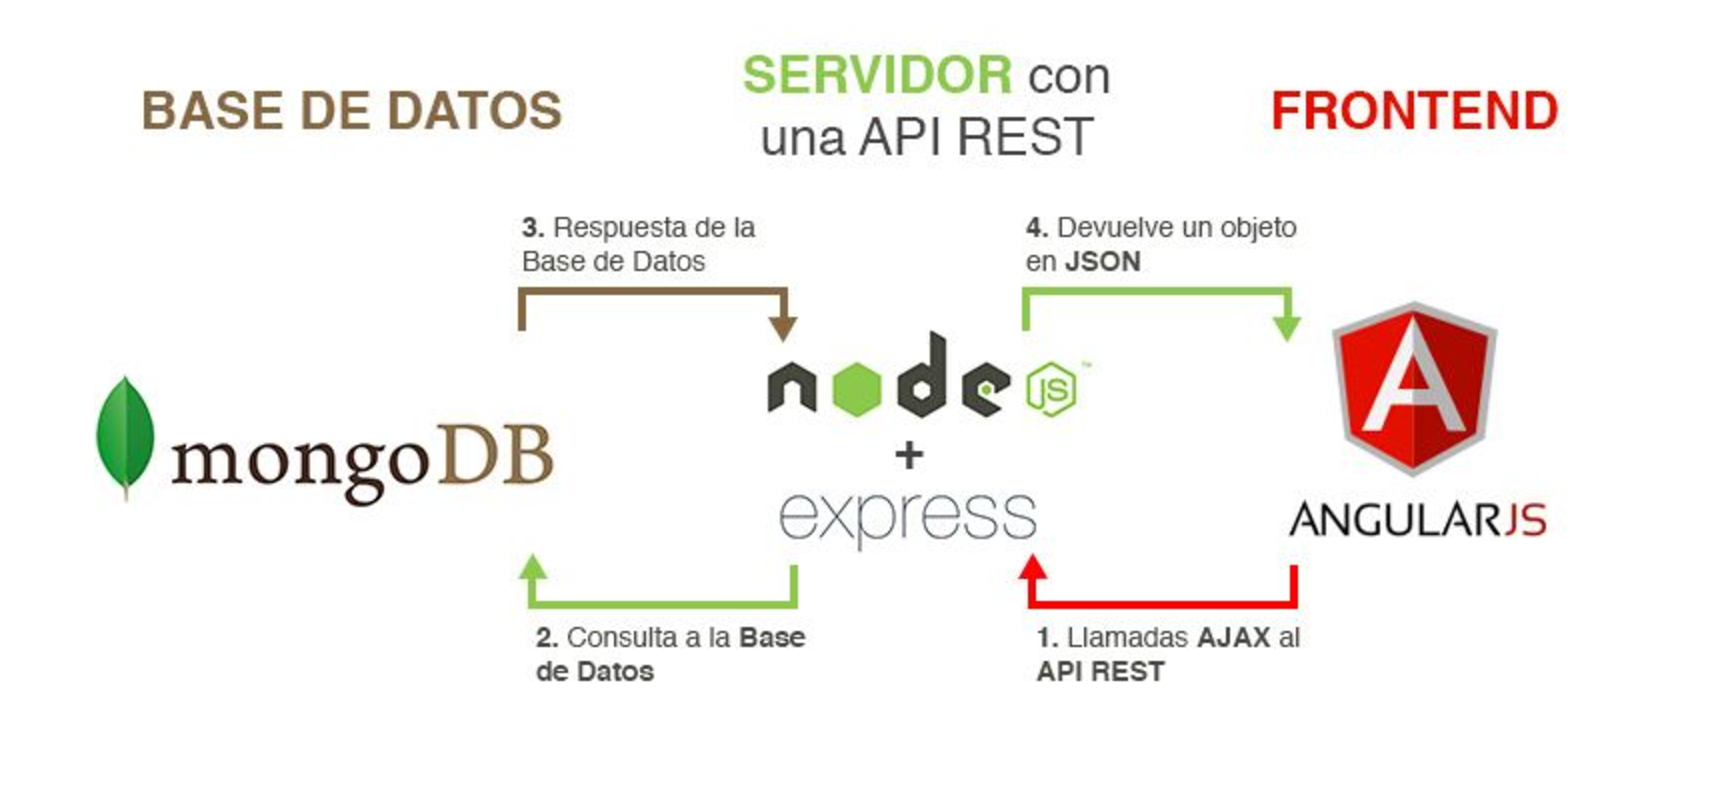
\includegraphics[width=140mm]{scheme.png}
    \caption{Esquema MEAN}
\end{figure}
En este esquema podemos ver como se comporta el stack MEAN, el cual hemos utilizado para el desarrollo de nuestra app. En este capítulo vamos a explicar como se comporta este paquete de 4 tecnologias: 


\section{MongoDB}
\begin{figure}[H]
    \centering
    
\includegraphics[width=40mm]{mongo.png}
\end{figure}
\subsection{Introduccion}

Mongo es una base de datos no relacional (NoSQL) de código abierto que guarda los datos en documentos tipo JSON (JavaScript Object Notation) pero en forma binaria (BSON) para hacer la integración de una manera más rápida. Se pueden ejecutar operaciones en JavaScript en su consola en lugar de consultas SQL. Además tiene una gran integración con Node.js con los driver propio y con Mongoose. Debido a su flexibilidad es muy escalable y ayuda al desarrollo ágil de proyectos web.

MongoDB esta orientado para servicios que necesiten una persistencia basada en documentos, al contrario que otros sistemas de base de datos noSQL como Cassandra, el cual esta orientado para logs, o como Redis que necesita una persistencia basada en colas de mensajes.

Estamos ante la era de lo que Martin Fowler llama “Polyglot
persistence”. Hay que decidir el tipo de persistencia a
utilizar para despues usar el tipo de persistencia que mas
se amolde a nuestras necesidades.

Las caracteristica que hacen tan importante a esta base de datos son las siguientes:



\begin{itemize}

    \item Está orientada a documentos. Lo que quiere decir que en un único documento es capaz de almacenar toda la información necesaria que define un producto, un cliente, etc, aceptando todo tipo de datos sin tener que seguir un esquema predefinido.
    
    \item Da respuesta a la necesidad de almacenamiento de todo tipo de datos: estructurados, semi estructurados y no estructurados. 
    
    \item Tiene un gran rendimiento en cuanto a escalabilidad y procesado de la información.
    
    \item Da respuesta a la necesidad de almacenamiento de todo tipo de datos: estructurados, semi estructurados y no estructurados. 
    
    \item Puede procesar la gran cantidad de información que se genera hoy en día..
    
    \item Permite a las empresas ser más ágiles y crecer más rápidamente, creando asi nuevos tipos de aplicaciones.
    
    
\end{itemize}

\subsection{MongoDB}

MongoDB esta escrito en C++, su version de 32 bits solo puede alcanzar 2GB, por este motivo la version de 32 bits no es recomendable usarla en produccion.
\begin{lstlisting}[language=JSON] 
{
    name: "mario",
    age: 24,
    preferences: [
        "programming",
        "nosql",
        "javascript"
    ]
}

\end{lstlisting}


Esto es un documento en Mongo, los cuales se almacenan en colecciones y estas a su vez en bases de datos. Estas colecciones poseen un esquema flexible y totalmente dinamico lo que hace que la velocidad de computo sea muy alta. Las bases de datos no se crean manualmente, primero se define la base de datos a usar y luego se inserta un documento en alguna coleccion.

\begin{lstlisting}[language=JSON] 
    > show dbs
    > use pruebanosql
    > show colections
    > db.users.insert({"name":"mario", "age":24})
\end{lstlisting}

Un problema que tiene Mongo, es que no soporta transacciones de multiples documentos, sin embargo puede proporciona operaciones atómicas en un solo documento. A menudo, estas operaciones atómicas de nivel de documento son suficientes para resolver los problemas que requerían transacciones en una base de datos relacional. Por ejemplo en Mongo se pueden incrustar datos relacionados en matrices anidadas o documentos anidados dentro de un solo documento y actualizar todo el documento en una sola operación atómica. Por este motivo los servicios que requieren de transacciones como los bancos o entidades economicas, no utilizan Mongo debido a que es sensible a Hacker, debido a que no es capaz de hacer una sola operación atomica en dos documentos.

Otro posible problema podria ser la excesiva cantidad de memoria RAM que puede consumir MongoDB, aunque es posible ejecutar mongo en una maquina con una pequeña cantidad de memoria RAM libre. Pero si es cierto que Mongo usa automaticamente toda la memoria libre del equipo como su cache, es por esto por lo que los monitores de recursos muestran que mongo utiliza una gran cantidad de memotria, pero su uso es dinámico. Es decir que si otro proceso de repente necesita mayor espacio de memoria RAM, MongoDB liberara parte de su memoria asignada para el otro proceso.

\subsection{Fragmentación (Sharding)}
\begin{figure}[H]
    \centering
    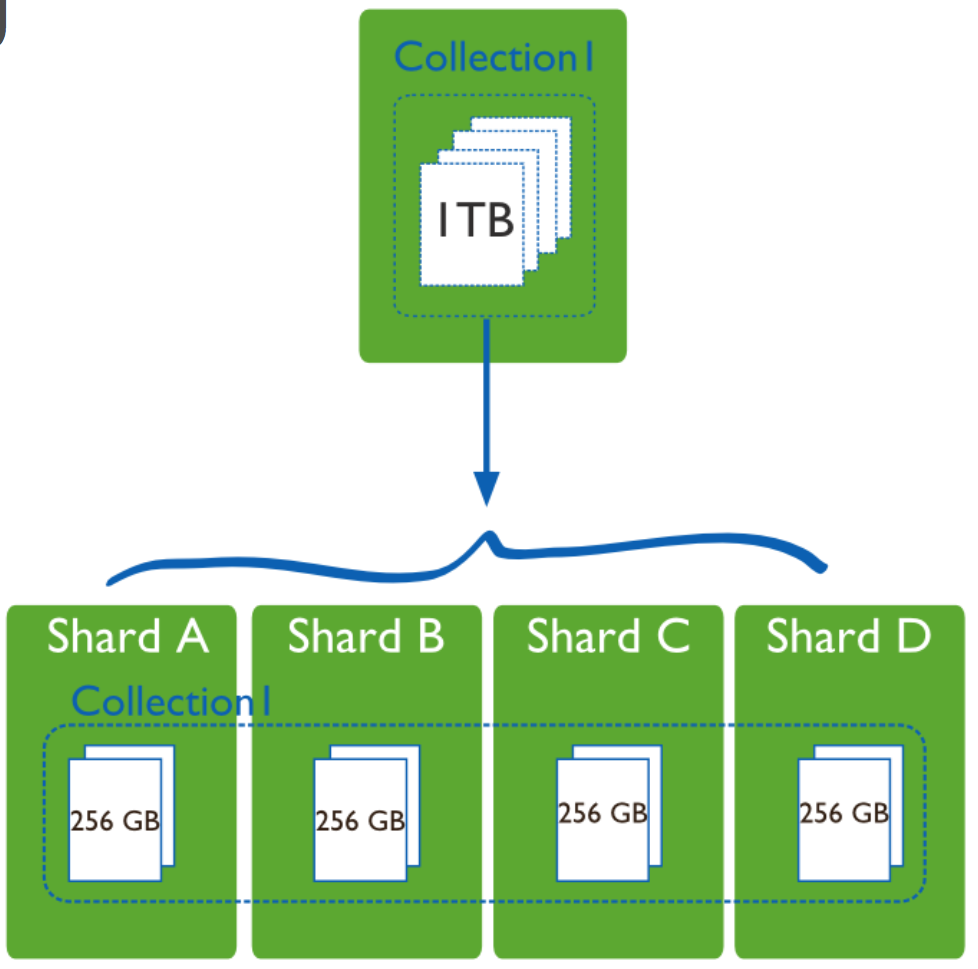
\includegraphics[width=90mm]{shard.png}
    \caption{Sharding}
\end{figure}
¿Que es el Sharding? Cuando el proyecto que estas llevando a cabo empieza a tener un numero de peticiones de acceso elevado , empiezas a notar que tu base de datos va mas lento de lo normal. Para este problema tienes dos soluciones, una actualizar toda la insfraestruztura para soportar la demanda o empezar a utilizar el sharding.

El sharding, es el modo en el que hacemos nuestra base de datos escalable. En lugar de tener una coleccion en una base de datos, la tendriamos en varias bases de datos distribuidas, de modo que a la hora de consultar los datos de dicha coleccion, los recuperaremos como si de una unica base de datos se tratase. Todo esto de encontrar la base de datos lo hace Mongo de forma transparente. Cuando hacemos consultas, tenemos un enrutador llamado "MongoS", el cual mantendra un pequeño pull de conexiones a los distintos host.

Los fragmentos estarán formados por replica set, de modo que
si creamos tres fragmentos, cada uno de los cuales tiene una
replica set con tres servidores, estaríamos hablando de un
total de nueve servidores. Para saber en que fragmento debe
consultar para recuperar datos de una coleccion ordenada, se
utilizan rangos y shard key, de modo que se torcea la colecicion en rangos y se les asigna un id a cada rango, de este modo que cuando se consulte la coleccion debemos proporcionar el "shard_Key".




\section{Express}

\begin{figure}[H]
    \centering
    
\includegraphics[width=90mm]{express.png}
\end{figure}

\subsection{Introduccion}
Express es un framework por encima de Node.js que permite crear servidores web y recibir peticiones HTTP de una manera sencilla, lo que permite también crear APIs REST de forma rápida.

Express es una plataforma ligera para construir aplicaciones web usando NodeJS. Nos ayuda a organizar las aplicaciones web en el lado del servidor. En la web de ExpressJS, lo describen como "un framework de desarrollo de aplicaciones web minimalista y flexible para Node.js". Sin duda el exito de express radica en lo sencillo que es usarlo, y además abarca un sin número de aspectos que muchos desconocen pero son necesarios.

De entre las tantas cosas que tiene este framework podemos destacar:

\begin{itemize}

\item \textbf{Router}
\item \textbf{Manejo de peticiones}
\item \textbf{Configuracion de la aplicacion}
\item \textbf{Middleware}
\end{itemize}

Para comenzar, y suponiendo que tienes ya instalado node y npm, lo único que es necesario hacer es lo siguiente:

\begin{lstlisting}[language=JSON] 
    > npm install -g express
\end{lstlisting}

Una vez instalado express puedes utilizar express NOMBRE-DEL-APP lo cual te creara una estructura personalizada y los archivos necesarios para comenzar a trabajar con el mismo. Haz cd NOMBRE-DEL-APP && npm install para instalar automaticamente las dependencias.

\subsection{Server.js}

En una aplicación escrita con express existe una estructura interna bien definida y es como sigue:


\begin{itemize}

    \item \textbf{Modúlos o archivos externos} Importamos todos los módulos o archivos externos que nuestra app vaya a necesitar. El bloque, o mejor dicho la línea, que viene a continuación es la más importante de todas, ya que se encarga de instanciar Express y asignarlo a la variable app, la cual se utilizará a partir de ahora para configurar los parámetros de Express.
    
    \begin{lstlisting}[language=JSON] 
    var app = express();
   \end{lstlisting}
   
   El siguiente bloque sirve para configurar e iniciar algunos componentes de Express. Destacar la línea, app.use(express.static(...)), en la cual se configuran los objetos estáticos (imágenes, hojas de estilo, etc.) que debe servir Express, los cuales se encuentran en la carpeta public. Esta configuración permite también que los elementos estáticos puedan ser accedidos como si se encontrasen en el directorio raíz del proyecto, de forma que para acceder a las imágenes ubicadas en /public/images se haría con la URL http://localhost:3000/images.
    \begin{lstlisting}[language=JSON] 
    app.use(bodyParser.json());
    app.use(bodyParser.urlencoded({ extended: false }));
    app.use(cookieParser());
    app.use(express.static(path.join(__dirname, 'public')));
   \end{lstlisting}
   
    
    \item \textbf{Conectamos a la base de datos} La segunda parte de nuesta app express, es conectarnos a la base datos. 
    
    \item \textbf{Importamos controladores y modelos de la base de datos} Una vez conectados a la base de datos importamos los controladores y los modelos de nuestra base de datos.
    
    
   \item \textbf{Rutas} Las rutas son definitivamente la parte más importante de tu aplicación, porque si estas no están definidas, no existiria una interfaz para él cliente.
   
   Como podemos ver una ruta esta especificada de la siguiente forma:
   \begin{lstlisting}[language=JSON] 
    app.VERBO(PATH, ACCION)
   \end{lstlisting}
   
   VERBO: Puede ser: GET, POST, PUT, DELETE y así para cada uno de los verbos HTTP. 
   
   PATH: Define la dirección de acceso.
   
   ACCION: Que es lo que se tiene que hacer.
   
   \item \textbf{Listen} Por último es importante que tu aplicación este disponible en algún puerto.
   \begin{lstlisting}[language=JSON] 
    app.listen(3000);
   \end{lstlisting}
   
\end{itemize}

Express esconde muchas funcionalidades internas de Node, lo que te permite sumergirte en el código de tu aplicación y conseguir tus objetivos de forma muy rápida. Es fácil de aprender y te deja cierta flexibilidad con su estructura.
Por algo es el framework más popular de Node. Algunos nombres destacados que usan Express son:

\begin{itemize}

\item \textbf{MySpace}
\item \textbf{LinkedIn}
\item \textbf{Segment.io}
\end{itemize}



\section{Angular 2}

\begin{figure}[H]
    \centering
    
\includegraphics[width=80mm]{a2.jpg}
\end{figure}


\subsection{Introduccion}

Angular 2 es un framework JS para la parte cliente o Frontend de una aplicación web, que respeta el paradigma MVC y permite crear Single-Page Applications (Aplicaciones web que no necesitan recargar la página), de manera más o menos sencilla. Es un proyecto mantenido por Google y que actualmente está muy en auge.

Para crear apps en Angular 2 necesitamos:

\begin{itemize}

\item \textbf{Componemos plantillas HTML (templates) con el markup de Angular 2}
\item \textbf{Escribimos Componentes para gestionar esas plantillas}
\item \textbf{Encapsulamos la lógica de la aplicación en Servicios}
\item \textbf{Entregamos el componente raíz de la app al sistema de arranque de Angular 2 (bootstrap).}
\end{itemize}

Veamos como se relacionan estos elementos en el diagrama de arquitectura típico, sacado de la web de Angular 2:

\begin{figure}[H]
    \centering
    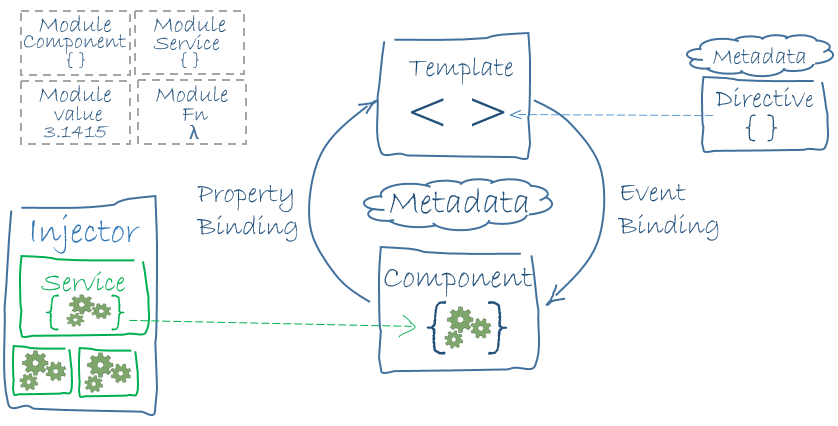
\includegraphics[width=110mm]{angular2Architecture.png}
\end{figure}

Podemos identificar los 8 bloques principales de una app con Angular 2:
\begin{itemize}

\item \textbf{Modulo} Igual que con su predecesor, las apps de Angular 2 son modulares. Un módulo, típicamente es un conjunto de código dedicado a cumplir un único objetivo. El módulo exporta algo representativo de ese código, típicamente una única cosa como una clase. Los modulos se pueden exportar e importar:

 \begin{lstlisting}[language=JSON] 
//app/app.component.js
    export class AppComponent {
        //aqui va la definicion del componente
    }
 
//app/main.js
    import { AppComponent } from './app.component';
\end{lstlisting}
   
Hay módulos que son librerías de conjuntos de módulos. Las librerías principales de Angular 2 son:
\begin{itemize}
\item \textbf{@angular/core}
\item \textbf{@angular/common}
\item \textbf{@angular/router}
\item \textbf{@angular/http}
\end{itemize}

\item \textbf{Componente} Un Component controla una zona de espacio de la pantalla que podríamos denominar vista. El componente define propiedades y métodos que están disponibles en su template, pero eso no te da licencia para meter ahí todo lo que te parezca. Haciendo un símil con AngularJS (Angular 1), un componente vendría a ser un controlador que siempre va ligado a una vista.
\item \textbf{Template} El Template (cuyo concepto ya existía en Angular 1), es lo que nos permite definir la vista de un Componente.
Igual que su predecesor, el template de Angular 2 es HTML, pero decorado con otros componentes y algunas directivas: expresiones de Angular que enriquecen el comportamiento del template.

Como vemos, además de elementos HTML normales como<h2> y <div>, hay otros elementos desconocidos en nuestro lenguaje de markup:
\begin{itemize}
\item \textbf{*ngForg}
\item \textbf{todo.subject}
\item \textbf{(click)}
\item \textbf{[todo]}
\item \textbf{todo-detail}
\end{itemize}

\item \textbf{Metadatos}
\item \textbf{Data Binding} Uno de los principales valores de Angular es que nos abstrae de la lógica pull/push asociada a insertar y actualizar valores en el HTML y convertir las respuestas de usuario (inputs, clicks, etc) en acciones concretas. Escribir toda esa lógica a mano (lo que típicamente se hacía con JQuery) es tedioso y propenso a errores, y Angular 2 lo resuelve por nosotros gracias al Data Binding.
\begin{itemize}
\item \textbf{Interpolación} Hacia el DOM.
{{todo.subject}}
\item \textbf{Property binding} Hacia el DOM. 
[todo]="selectedTodo"
\item \textbf{Event binding} Desde el DOM. (click)="selectTodo(todo)"

\item \textbf{Two-way binding} (Desde/Hacia el DOM) input [(ngModel)]="todo.subject"
\end{itemize}
\item \textbf{Directiva}
\item \textbf{Servicio}
\item \textbf{Dependency Injection}  Una dependencia en tu código se produce cuando un objeto depende de otro. Hay diferentes grados de dependencia, pero tenerla en exceso hace que testear tu código sea complicado o que algunos procesos se ejecuten más tiempo de la cuenta.
La inyección de dependencias es un método por el cual damos a un objeto las dependencias que requiere para su funcionamiento. 
\end{itemize}

Angular permite extender el vocabulario de tu HTML con directivas y atributos para crear componentes dinámicos. Si alguna vez has hecho una página web dinámica sin Angular te habrás dado cuenta de ciertas complicaciones frecuentes, como el data binding, validación de formulario, manejador de eventos con DOM (Document Object Model) y otras muchas. Angular presenta una solución “todo-en-uno” a esos problemas.
La curva de aprendizaje para Angular es muy pequeña, lo que explica que mucha gente se este pasando a este framework. La sintaxis es simple y sus principios básicos como el data binding (vinculación de elementos de nuestro documento HTML con nuestro modelo de datos) y la inyección de dependencias son sencillas de entender.

\begin{itemize}



\end{itemize}

\section{Node}

\begin{figure}[H]
    \centering
    
\includegraphics[width=80mm]{node.png}

\end{figure}
Node es un entorno de programación en JavaScript para el Backend basado en el motor V8 de JavaScript del navegador Google Chrome y orientado a eventos, no bloqueante, lo que lo hace muy rápido a la hora de crear servidores web y emplear tiempo real. Fue creado en 2009 y aunque aún es joven, las últimas versiones lo hacen más robusto además de la gran comunidad de desarrolladores que posee.

\begin{itemize}
\item \textbf{NPM}.Uno de los beneficios de Node es su gestor de paquetes, npm (node package manager) y nos permite gestionar todas las dependencias y módulos de una aplicación. Al igual que Ruby tiene RubyGems y PHP tiene Composer, Node tiene npm.
Viene ya incluido con Node y permite que nos bajemos una serie de packages/paquetes para satisfacer nuestras necesidades. Los packages amplían la funcionalidad de Node y este sistema de paquetes una de las cosas que hace a Node tan potente.
La capacidad de tener una serie de códigos que puedes reutilizar en todos tus proyectos es increíble y hace que el desarrollo sea mucho más sencillo. Puedes combinar varios paquetes para crear aplicaciones complejas.
\end{itemize}


\end{document}



